\documentclass[11pt,oneside]{article}    %use"amsart"insteadof"article"forAMSLaTeXformat
\usepackage{geometry}        %Seegeometry.pdftolearnthelayoutoptions.Therearelots.
\geometry{letterpaper}        %...ora4paperora5paperor...
%\geometry{landscape}        %Activateforforrotatedpagegeometry
%\usepackage[parfill]{parskip}        %Activatetobeginparagraphswithanemptylineratherthananindent
\usepackage{graphicx}                %Usepdf,png,jpg,orepsßwithpdflatex;useepsinDVImode
                                %TeXwillautomaticallyconverteps-->pdfinpdflatex        
\usepackage{amssymb}
\usepackage[colorlinks]{hyperref}

%----macros begin---------------------------------------------------------------
\usepackage{color}
\usepackage{amsthm}

\def\conv{\mbox{\textrm{conv}\,}}
\def\aff{\mbox{\textrm{aff}\,}}
\def\E{\mathbb{E}}
\def\R{\mathbb{R}}
\def\Z{\mathbb{Z}}
\def\tex{\TeX}
\def\latex{\LaTeX}
\def\v#1{{\bf #1}}
\def\p#1{{\bf #1}}
\def\T#1{{\bf #1}}

\def\vet#1{{\left(\begin{array}{cccccccccccccccccccc}#1\end{array}\right)}}
\def\mat#1{{\left(\begin{array}{cccccccccccccccccccc}#1\end{array}\right)}}

\def\lin{\mbox{\rm lin}\,}
\def\aff{\mbox{\rm aff}\,}
\def\pos{\mbox{\rm pos}\,}
\def\cone{\mbox{\rm cone}\,}
\def\conv{\mbox{\rm conv}\,}
\newcommand{\homog}[0]{\mbox{\rm homog}\,}
\newcommand{\relint}[0]{\mbox{\rm relint}\,}

%----macros end-----------------------------------------------------------------

\title{Boolean chains
\footnote{This document is part of the \emph{Linear Algebraic Representation with CoChains} (LAR-CC) framework~\cite{cclar-proj:2013:00}. \today}
}
\author{Alberto Paoluzzi}
%\date{}                            %Activatetodisplayagivendateornodate

\begin{document}
\maketitle
\nonstopmode

\begin{abstract}
A novel algorithm for computation of Boolean operations between cellular complexes is given in this module.
It is based on bucketing of possibly interacting geometry using a box-extension of kd-trees, normally used for  point proximity queries. 
Such kd-tree representation of containment boxes of cells, allow us to compute a number of independent buckets of data to be used for local intersection, followed by elimination of duplicated data.
Actually we reduce the intersection of boundaries in 3D to the independent intersections of the buckets of (transformed) faces with the 2D subspace $z=0$, in order to reconstruct each splitted facet of boolean arguments, suitably transformed ther together with the bucket of indent facets.
A final tagging of cells as either belonging or not to each operand follows, allowing for fast extraction of Boolean results between any pair of chains (subsets of cells).
This Boolean algorithm can be considered of a \emph{Map-Reduce} kind, and hence suitable of a distributed implementation over big datasets. The actual engineered implementation will follow the present prototype, using some distributed NoSQL database, like MongoDB or Riak. 
\end{abstract}

\tableofcontents

%===============================================================================
\section{Introduction}
%===============================================================================


%===============================================================================
\section{Preview of the algorithm}
%===============================================================================

The whole Boolean algorithm is composed by four stages in sequence, denoted in the following as \emph{Unification}, \emph{Bucketing}, \emph{Intersection}, and \emph{Reconstruction}. The algorithm described here is both multidimensional and variadic. Multidimensional means that the arguments are solid in Euclidean space of dimension $d$, with $d$ small integer.
The \emph{arity}  of a function or operation is the number of arguments or operands the function or operation accepts. 
In computer science, a function accepting a variable number of arguments is called \emph{variadic}.

\subsection{Unification}
%===============================================================================

In this first step the boundaries of the $n$ Boolean arguments are computed and merged together as a set of chains defined in the discrete set $\texttt{V}$ made by the union of their vertices, and possibly by a discrete set of points generated by intersection of cells of complementary dimension, i.e. whose dimensions add up to the dimension of the ambient space.
Actually, only the (\emph{oriented}) boundaries \texttt{V,FV$_i$} $(1\leq i\leq n)$ of the varius arguments are retained here, and used by the following steps of the algorithm.

\subsection{Bucketing}
%===============================================================================

The bounding boxes of facets \texttt{FV$_i$} are computed, and their \emph{box-kd-tree} is worked-out, so providing a group of buckets of close cells, that can be elaborated independently, and possibly in parallel, to compute the intersections of the boundary cells. 

\subsection{Intersection}
%===============================================================================

For each facet $f$ of one of Boolean arguments, the subset $F(f)$ of incident or intersecting facets of boundaries of the other arguments were computed in the previous \emph{bucketing} step. So, each $F$ is transformed by the affine map that sends $f$ into the $z=0$ subspace, and there is intersected with this subspace, generating a subset $E(f)$ of coplanar edges.
This one is projected in 2D, and the \emph{regularized} cellular 2-complex $G(f)$ induced by it is computed, and mapped back to the original space position and orientation of $f$ (providing a partition of it induced by the other boundaries).

\subsection{Reconstruction}
%===============================================================================

Like for in the reconstruction of 2D solid cells using the angular ordering of edges around the vertices, the coincident edges are identified in 3D , and used to sort the incident faces sing vhe falues of solid angles given with one reference face.
The 3D space partition induced by $\cup_f G(f)$ is finally reconstructed, possibly in parallel, by traversing the adjacent sets of facets on the boundary of each solid cell.



%===============================================================================
\section{Implementation}
%===============================================================================

\subsection{Box-kd-tree}
%===============================================================================


\paragraph{Split the boxes between the (below,above) subsets}
%-------------------------------------------------------------------------------
@D Split the boxes between the below,above subsets
@{""" Split the boxes between the below,above subsets """
def splitOnThreshold(boxes,subset,coord):
    theBoxes = [boxes[k] for k in subset]
    threshold = centroid(theBoxes,coord)
    ncoords = len(boxes[0])/2
    a = coord%ncoords
    b = a+ncoords
    below,above = [],[]
    for k in subset:
        if boxes[k][a] <= threshold: below += [k]
    for k in subset:
        if boxes[k][b] >= threshold: above += [k]
    return below,above
@}
%-------------------------------------------------------------------------------

\paragraph{Test if bucket OK or append to splitting stack}
%-------------------------------------------------------------------------------
@D Test if bucket OK or append to splitting stack
@{""" Test if bucket OK or append to splitting stack """
def splitting(bucket,below,above, finalBuckets,splittingStack):
    if (len(below)<4 and len(above)<4) or len(set(bucket).difference(below))<7 \
        or len(set(bucket).difference(above))<7: 
        finalBuckets.append(below)
        finalBuckets.append(above)
    else: 
        splittingStack.append(below)
        splittingStack.append(above)
@}
%-------------------------------------------------------------------------------


\paragraph{Remove subsets from bucket list}
%-------------------------------------------------------------------------------
@D Remove subsets from bucket list @{
""" Remove subsets from bucket list """
def removeSubsets(buckets):
    n = len(buckets)
    A = zeros((n,n))
    for i,bucket in enumerate(buckets):
        for j,bucket1 in enumerate(buckets):
            if set(bucket).issubset(set(bucket1)):
                A[i,j] = 1
    B = AA(sum)(A.tolist())
    out = [bucket for i,bucket in enumerate(buckets) if B[i]==1]
    return out

def geomPartitionate(boxes,buckets):
    geomInters = [set() for h in range(len(boxes))]
    for bucket in buckets:
        for k in bucket:
            geomInters[k] = geomInters[k].union(bucket)
    for h,inters in enumerate(geomInters):
        geomInters[h] = geomInters[h].difference([h])
    return AA(list)(geomInters)
@}
%-------------------------------------------------------------------------------
    


\paragraph{Iterate the splitting until \texttt{splittingStack} is empty}
%-------------------------------------------------------------------------------
@D Iterate the splitting until splittingStack is empty
@{""" Iterate the splitting until \texttt{splittingStack} is empty """
def boxTest(boxes,h,k):
    B1,B2,B3,B4,B5,B6,_ = boxes[k]
    b1,b2,b3,b4,b5,b6,_ = boxes[h]
    return not (b4<B1 or B4<b1 or b5<B2 or B5<b2 or b6<B3 or B6<b3)

def boxBuckets(boxes):
    bucket = range(len(boxes))
    splittingStack = [bucket]
    finalBuckets = []
    while splittingStack != []:
        bucket = splittingStack.pop()
        below,above = splitOnThreshold(boxes,bucket,1)
        below1,above1 = splitOnThreshold(boxes,above,2)
        below2,above2 = splitOnThreshold(boxes,below,2) 
               
        below11,above11 = splitOnThreshold(boxes,above1,3)
        below21,above21 = splitOnThreshold(boxes,below1,3)        
        below12,above12 = splitOnThreshold(boxes,above2,3)
        below22,above22 = splitOnThreshold(boxes,below2,3)  
              
        splitting(above1,below11,above11, finalBuckets,splittingStack)
        splitting(below1,below21,above21, finalBuckets,splittingStack)
        splitting(above2,below12,above12, finalBuckets,splittingStack)
        splitting(below2,below22,above22, finalBuckets,splittingStack)
        
        finalBuckets = list(set(AA(tuple)(finalBuckets)))
    parts = geomPartitionate(boxes,finalBuckets)
    parts = [[h for h in part if boxTest(boxes,h,k)] for k,part in enumerate(parts)]
    return AA(sorted)(parts)
@}
%-------------------------------------------------------------------------------

\paragraph{aaaaaa}
%-------------------------------------------------------------------------------
@D aaaaaa
@{""" aaaaa """

@}
%-------------------------------------------------------------------------------


\subsection{Merging the boundaries}
%===============================================================================

\subsection{Elementary splitting}
%===============================================================================

In this section we implement the splitting of $(d-1)$-faces, stored in \texttt{FV}, induced by the buckets of $(d-1)$-faces, stored in \texttt{parts}, and one-to-one associated to them. Of course, (a) both such arrays have the same number of elements, and (b) whereas \texttt{FV} contains the indices of incident vertices for each face, \texttt{parts}  contains the indices of adjacent faces for each face, with the further constraint that $i \not\in \texttt{parts}(i)$.

\paragraph{Computation of topological relations} 
The function \texttt{crossRelation} is used here to compute a topological relation starting from two characteristic matrices \texttt{XV} and \texttt{YV}, that associate the sets of topological objects $X$ and $Y$ with their vertices, respectively.
The technique using sparse binary matrices stored in \texttt{CSR} (Compressed Sparse Row) format is used.

%-------------------------------------------------------------------------------
@D Computation of topological relation
@{""" Computation of topological relation """
def crossRelation(XV,YV):
    csrXV = csrCreate(XV)
    csrYV = csrCreate(YV)
    csrXY = matrixProduct(csrXV, csrYV.T)
    XY = [None for k in range(len(XV))]
    for k,face in enumerate(XV):
        data = csrXY[k].data
        col = csrXY[k].indices
        XY[k] = [col[h] for h,val in enumerate(data) if val==2] 
        # NOTE: val depends on the relation under consideration ...
    return XY
@}
%-------------------------------------------------------------------------------
    
\paragraph{Submanifold mapping computation}
The $4\times 4$ (affine) scipy matrix \texttt{transform} of type \texttt{mat} is computed by the function \texttt{submanifoldMapping}, using as input the array \texttt{pivotFace} that contains the vertices of the so-called \emph{pivot} face, i.e.~of the face to be mapped to the coordinate subspace $z=0$ (in 3D).

%-------------------------------------------------------------------------------
@D Submanifold mapping computation
@{""" Submanifold mapping computation """
def submanifoldMapping(pivotFace):
    tx,ty,tz = pivotFace[0]
    transl = mat([[1,0,0,-tx],[0,1,0,-ty],[0,0,1,-tz],[0,0,0,1]])
    facet = [ VECTDIFF([v,pivotFace[0]]) for v in pivotFace ]
    m = faceTransformations(facet)
    mapping = mat([[m[0,0],m[0,1],m[0,2],0],[m[1,0],m[1,1],m[1,2],0],[m[2,0],
                    m[2,1],m[2,2],0],[0,0,0,1]])
    transform = mapping * transl
    return transform
@}
%-------------------------------------------------------------------------------

\paragraph{Set of line segments partitioning a facet}
The more important function of this section is the higher level \texttt{intersection} function, that accepts as input the \texttt{LAR} model \texttt{(V,FV,EV)} to be partitioned, and the pair \texttt{(k,bundledFaces)}, where \texttt{k} is the index of the pivot face (to be transformed to the $z=0$ subspace) and where \texttt{bundledFaces} is an array of indices of faces that are guarantee to share points with face $k$. Such shared points may be either boundary edges of $k$ or a segment that is internal both to face $k$ and to some face in  \texttt{bundledFaces}.

%-------------------------------------------------------------------------------
@D Set of line segments partitioning a facet
@{""" Set of line segments partitioning a facet """
def intersection(V,FV,EV):
    FE = crossRelation(FV,EV)

    def intersection0(k,bundledFaces):
        pivotFace = [V[v] for v in FV[k]]
        transform = submanifoldMapping(pivotFace)  # submanifold transformation
        transformedCells,edges,faces = [],[],[]
        for face in bundledFaces:
            edge = set(FE[k]).intersection(FE[face])  # common edge index
            if edge == set():
                candidateEdges = FE[face]
                facet = []
                for e in candidateEdges:
                    cell = [V[v]+[1.0] for v in EV[e]]  # verts of incident face
                    transformedCell = (transform * (mat(cell).T)).T.tolist()  
                    # vertices in local frame
                    facet += [[point[:-1] for point in transformedCell]]
                faces += [facet]
            else:  # boundary edges of face k
                e, = edge
                vs = [V[v]+[1.0] for v in EV[e]]
                ws = (transform * (mat(vs).T)).T.tolist()
                edges += [[p[:-1] for p in ws]]
        return edges,faces,transform
    return intersection0    
@}
%-------------------------------------------------------------------------------



\paragraph{Computation of face transformations}
The faces in every $\texttt{parts}(i)$ must be affinely transformed into the subspace $x_d=0$, in order to compute the intersection of its elements with this subspace, that are submanifolds of dimension $d-2$.

%-------------------------------------------------------------------------------
@D Computation of face transformations
@{""" Computation of affine face transformations """
from scipy.linalg.basic import det

def COVECTOR(points):
    pointdim = len(points[0])
    plane = Planef.bestFittingPlane(pointdim,
                    [item for sublist in points for item in sublist])
    return [plane.get(I) for I in range(0,pointdim+1)]

def faceTransformations(facet):
    covector = COVECTOR(facet)
    translVector = facet[0]
    # translation 
    newFacet = [ VECTDIFF([v,translVector]) for v in facet ]
    # linear transformation: boundaryFacet -> standard (d-1)-simplex
    d = len(facet[0])
    m = mat( newFacet[1:d] + [covector[1:]] )
    if det(m)==0.0:
        for k in range(len(facet)-2):
            m = mat( newFacet[1+k+1:d+k+1] + [covector[1:]] )
            if det(m)!=0.0: break
    transformMat = m.T.I
    # transformation in the subspace x_d = 0
    out = (transformMat * (mat(newFacet).T)).T.tolist()
    return transformMat
@}
%-------------------------------------------------------------------------------
    
    

\paragraph{Space partitioning via submanifold mapping}

the function \texttt{spacePartition}, given in the below script, takes as input a \emph{non-valid} (with the meaning used in solid modeling field --- see~\cite{Requicha:1980:RRS:356827.356833}) \texttt{LAR} model of dimension $d-1$, i.e.~a triple \texttt{(V,FV,EV)}, and an array \texttt{parts} indexed on faces, and containing the subset of faces with greatest probability of intersecting each indexing face, respectively. The \texttt{spacePartition} function returns the \emph{valid} \texttt{LAR} boundary model \texttt{(W,FW,EW)} of the space partition induced by \texttt{FV}.
 
%-------------------------------------------------------------------------------
@D Space partitioning via submanifold mapping
@{@< Take the two extremes of a set of aligned points @>

""" Space partitioning via submanifold mapping """
def spacePartition(V,FV,EV, parts):
    transfFaces = []
    splitting = intersection(V,FV,EV)
    for k,bundledFaces in enumerate(parts):
        edges,faces,transform = splitting(k,bundledFaces)
        if DEBUG:
            print "\nk,bundledFaces =",k,",",bundledFaces
            print "edges =",edges
            print "faces =",faces
            print "transform =",transform
            VV = AA(LIST)(range(len(V)))
            submodel = STRUCT(MKPOLS((V,EV)))
            VIEW(larModelNumbering(1,1,1)(V,[VV,EV,FV],submodel,0.6)) 
        for face in faces:
            line = []
            for edge in face:
                (x1,y1,z1),(x2,y2,z2) = edge
                if not verySmall(z2-z1):
                    x = (x2-x1)/(z2-z1) + x1
                    y = (y2-y1)/(z2-z1) + y1
                    p = [x,y,0]
                    line += [eval(vcode(p))]
            if line!=[]: 
                if len(line)==2: edges += [line]
                elif len(line)>2: edges += takeExtremePoints(line)
                else: print "error: too few points in line"
            
        if DEBUG: print "> edges =",edges
        edges = [[point[:-1] for point in edge] for edge in edges]
        edges = AA(AA(eval))(AA(AA(vcode))(edges))
        if DEBUG: print "< edges =",edges
        v,fv,ev = larFromLines(edges) 
        if DEBUG:
            print "k,v,fv,ev =",k,v,fv,ev ,"\n"
            VIEW(SKEL_1(EXPLODE(1.2,1.2,1.2)(MKPOLS((v,ev)))))
        if len(fv)>1: fv = fv[:-1]   ## ??
        lar = [w+[0.0] for w in v],fv,ev
        transfFaces += [Struct([ larApply(transform.I)(lar) ])]
    W,FW,EW = struct2lar(Struct(transfFaces))
    #FW,EW = edgeCheck(W,FW,EW)
    return W,FW,EW
@}
%-------------------------------------------------------------------------------

%\paragraph{Take the two extremes of a set of aligned 2D points}
%The function \texttt{takeExtremePoints} is used to compute the two extreme points from a list, names \texttt{line} of aligned points. For this purpose the first and last list elements are used to define the parametric equation of the \emph{aligned set}:
%\[
%\p{p}=\p{p}_1+ \alpha (\p{p}_2-\p{p}_1),\quad\mbax{so that}\quad
%\alpha = (\p{p}-\p{p}_1)/(\p{p}_2-\p{p}_1).
%\] 
%The substitution of every point in \texttt{line} in the above formula is used to compute their corresponding parameter values, which are finally sorted to get the extreme points.

%-------------------------------------------------------------------------------
@D Take the two extremes of a set of aligned points
@{""" Take the two extremes of a set of aligned points """
def takeExtremePoints(line):
    [x1,y1,z1],[x2,y2,z1] = line[0], line[-1]
    if x1 != x2: parameters = [(x-x1)/(x2-x1) for x,y,z in line]
    elif y1 != y2: parameters = [(y-y1)/(y2-y1) for x,y,z in line]
    pairs = sorted(zip(parameters,line))
    """
    p_first = pairs[0][1]
    p_last = pairs[-1][1]
    return [p_first,p_last]
    """
    edges = [[pairs[k][1],pairs[k+1][1]] for k,pair in enumerate(pairs[:-1])]
    return edges
@}
%-------------------------------------------------------------------------------


\paragraph{Check for superimposing edges}
%-------------------------------------------------------------------------------
@D Check for superimposing edges
@{""" Check for superimposing edges """
def edgeCheck(V,FV,EV):
    VE = invertRelation(EV)
    EF = crossRelation(EV,FV)
    tripleVerts2e = defaultdict(list)
    for e,(v1,v2) in enumerate(EV):
        V1 = set(CAT([EV[edge] for edge in VE[v1]])) 
        V2 = set(CAT([EV[edge] for edge in VE[v2]])) 
        commonVerts = V1.intersection(V2)
        tripleVerts2e[tuple(sorted(commonVerts))] += [e]
    EW = []
    for verts,edges in tripleVerts2e.items():
        print verts,edges
        if len(edges)==1:  EW += [verts]
        elif len(edges)==3: 
            sizes = [VECTNORM(VECTDIFF([V[v] for v in EV[e]])) for e in edges]
            _,theEdge = max(zip(sizes,edges))
            addedVert = list(set(verts).difference(EV[theEdge]))[0]
            for face in EF[theEdge]:
                if addedVert not in FV[face]:  
                    newList = list(FV[face])+[addedVert]
                    FV[face] = tuple(newList)
            if sizes[0] == ABS(sizes[1]-sizes[2]): EW += [EV[edges[0]]]
            if sizes[1] == ABS(sizes[2]-sizes[0]): EW += [EV[edges[1]]]
            if sizes[2] == ABS(sizes[0]-sizes[1]): EW += [EV[edges[2]]]
        else: print "error: in edgeCheck"
    return FV,EW
@}
%-------------------------------------------------------------------------------


\subsection{Circular ordering of faces around edges}


\paragraph{Directional and orthogonal projection operators}

In order to sort circularly the faces incident on each edge, we need of course to compute the relation EF, and for each face $f$ incident on $e = (v_1,v_2)$, to project a vector $w_f = (v_1,v_f)$, non parallel to $(v_1,v_2)$, on the subspace ortogonal to $e$. This may be done by mapping $w_f$ with the tensor $I-e \otimes e$. Finally, the angles between vectors $a,b$ in this orthogonal space to $e$ may be computed by using the \texttt{atan2} function, that combines both the $sin$ and the $cos$ of the angle:
\[
angle = atan2(norm(cross(a,b)),dot(a,b)).
\]
Let us just remember that, by definition, $(e \otimes e)v = (e \cdot v)e$, where $e,v$ are vectors.
%-------------------------------------------------------------------------------
@D Directional and orthogonal projection operators
@{""" Directional and orthogonal projection operators """
def dirProject (e):
    def dirProject0 (v):
        return SCALARVECTPROD([ INNERPROD([ UNITVECT(e), v ]), UNITVECT(e) ])
    return dirProject0

def orthoProject (e):
    def orthoProject0 (v):  
        return VECTDIFF([ v, dirProject(UNITVECT(e))(v) ])
    return orthoProject0
@}
%-------------------------------------------------------------------------------




\paragraph{3D boundary triangulation of the space partition}
The function \texttt{boundaryTriangu\-la\-tion} given below is used to guarantee that there is a unique (simple) facet incident to an edge and contained in one LAR facet. More clearly, the Boolean decompositions generated by LAR allow for non convex cells, and in particular for nonconvex boundary facets of $d$-cells. This fact may induce errors in the computation of circularly sorted faces around edges. Conversely, by decomposing the faces into triangles, such ordering problems cannot appear.  
We also note that whereas every $(d-1)$-facet is made by coherently oriented triangles, it is not possible to give---a priori---a coherently orientation to all the facets, since the object interior and exterior are not defined (for now).

%-------------------------------------------------------------------------------
@D 3D boundary triangulation of the space partition 
@{from support import PolygonTessellator,vertex

def orientTriangle(pointTriple):
    v1 = array(pointTriple[1])-pointTriple[0]
    v2 = array(pointTriple[2])-pointTriple[0]
    if cross(v1,v2)[2] < 0: return REVERSE(pointTriple)
    else: return pointTriple
    
from triangle import triangulate
from copy import copy
def boundaryTriangulation(W,FW,EW,FE):
    triangleSet = []    
    for f,face in enumerate(FW):
        edges = FE[f]
        pivotFace = [W[v] for v in face]
        transform = submanifoldMapping(pivotFace)
        mappedVerts = (transform * (mat([p+[1.0] for p in pivotFace]).T)).T.tolist()
        verts2D = [point[:-2] for point in mappedVerts]  
        pts = array(verts2D)
        n = len(verts2D)
        EdgeVerts = AA(list)(zip(range(n),range(1,n)+[0]))
        tri = {    'vertices': pts, 'segments': EdgeVerts }
        triangles = triangulate(tri)['triangles'].tolist()
        pts = pts.tolist()
        
        centers = [CCOMB([pts[v] for v in triangle]) for triangle in triangles]
        triangles = [triangle for triangle,p in zip(triangles,centers) 
        	if pointInPolygonClassification(p,(pts,EdgeVerts))=="p_in"]	

        points = (transform.I * (mat(mappedVerts).T)).T.tolist()
        trias = [[points[k][:-1] for k in face]+[points[face[0]][:-1]] for face in triangles]
        triangleSet += [AA(orientTriangle)(trias)]
    return triangleSet

def triangleIndices(triangleSet,W):
    vertDict,out = defaultdict(),[]
    for k,vertex in enumerate(W):  vertDict[vcode(vertex)] = k
    for h,faceSetOfTriangles in enumerate(triangleSet):
        trias = [[vertDict[vcode(p)] for p in triangle[:-1]] 
                    for triangle in faceSetOfTriangles]
        out += [trias]
    return out
@}
%-------------------------------------------------------------------------------


\paragraph{Computation of incidence between edges and 3D triangles}
%-------------------------------------------------------------------------------
@D Computation of incidence between edges and 3D triangles @{
def edgesTriangles(EF, FW, TW, EW):
    ET = [None for k in range(len(EF))]
    for e,edgeFaces in enumerate(EF):
        ET[e] = []
        for f in edgeFaces:
            for t in TW[f]:
                if set(EW[e]).intersection(t)==set(EW[e]):
                    ET[e] += [t]
    return ET
@}
%-------------------------------------------------------------------------------

\begin{figure}[htbp] %  figure placement: here, top, bottom, or page
   \centering
   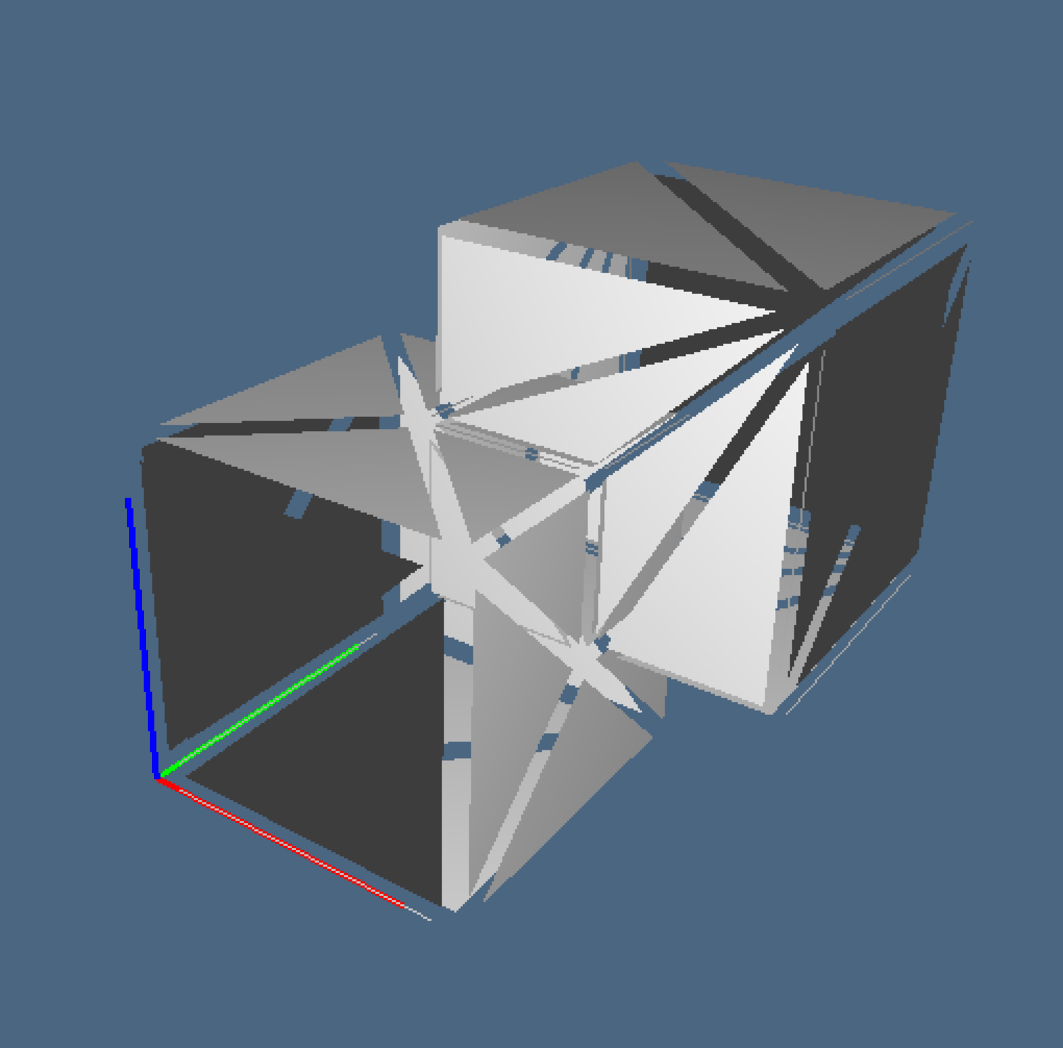
\includegraphics[height=0.325\linewidth,width=0.325\linewidth]{images/3Dtriangulation} 
   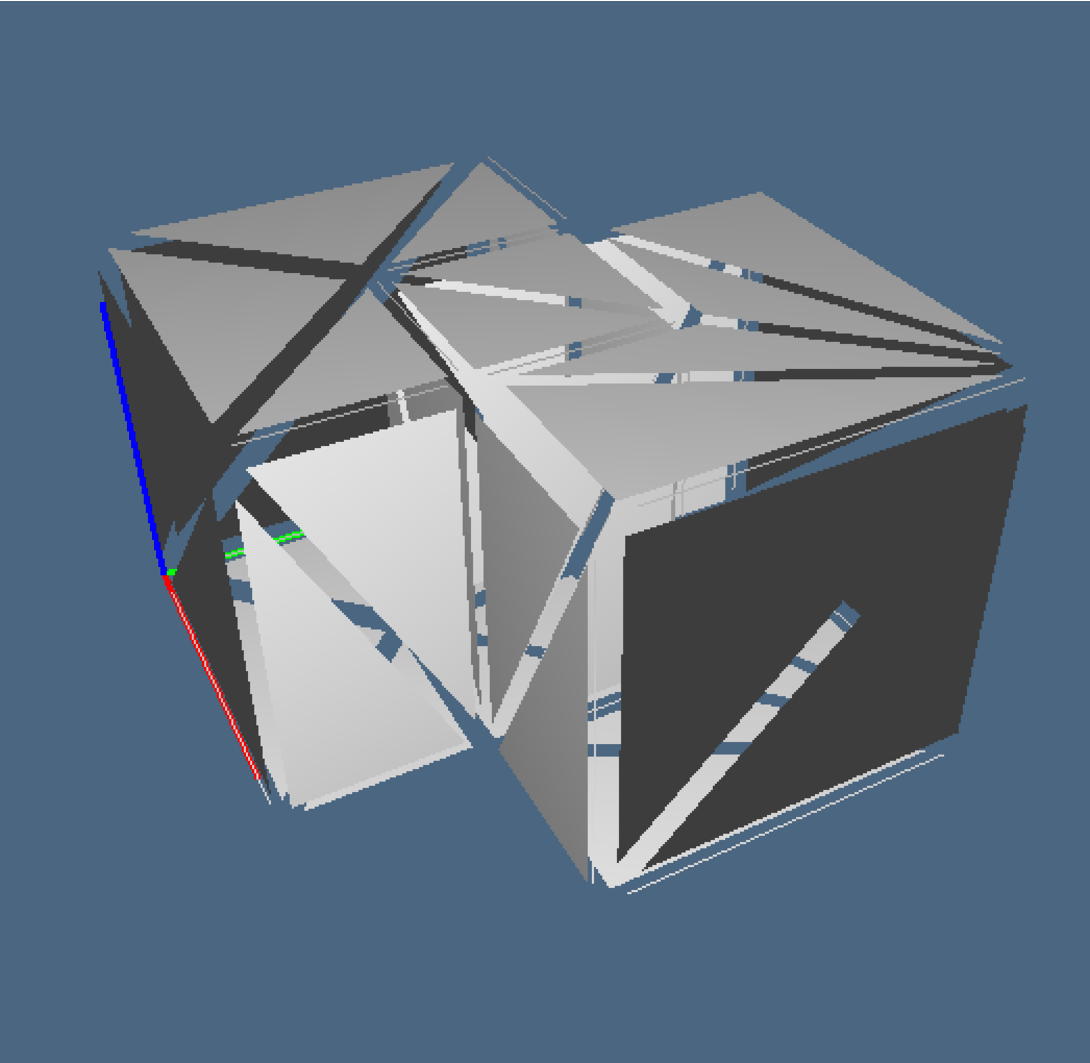
\includegraphics[height=0.325\linewidth,width=0.325\linewidth]{images/3Dtriangulation2} 
   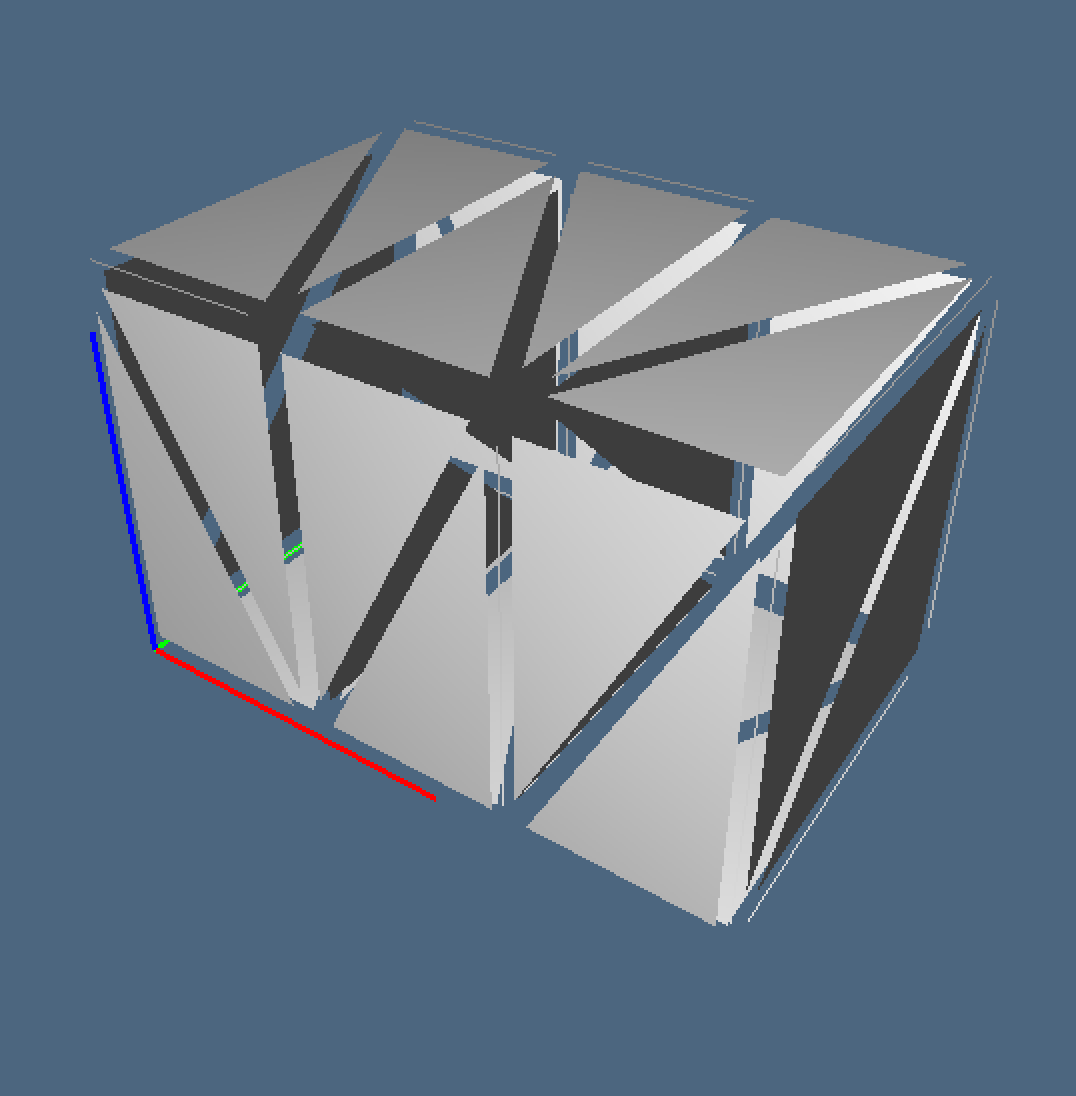
\includegraphics[height=0.325\linewidth,width=0.325\linewidth]{images/3Dtriangulation3} 
   \caption{The triangulated boundaries of the space partition induced by two cubes (one is variously translated).}
   \label{fig:3Dtriangulation}
\end{figure}

\begin{figure}[htbp] %  figure placement: here, top, bottom, or page
   \centering
   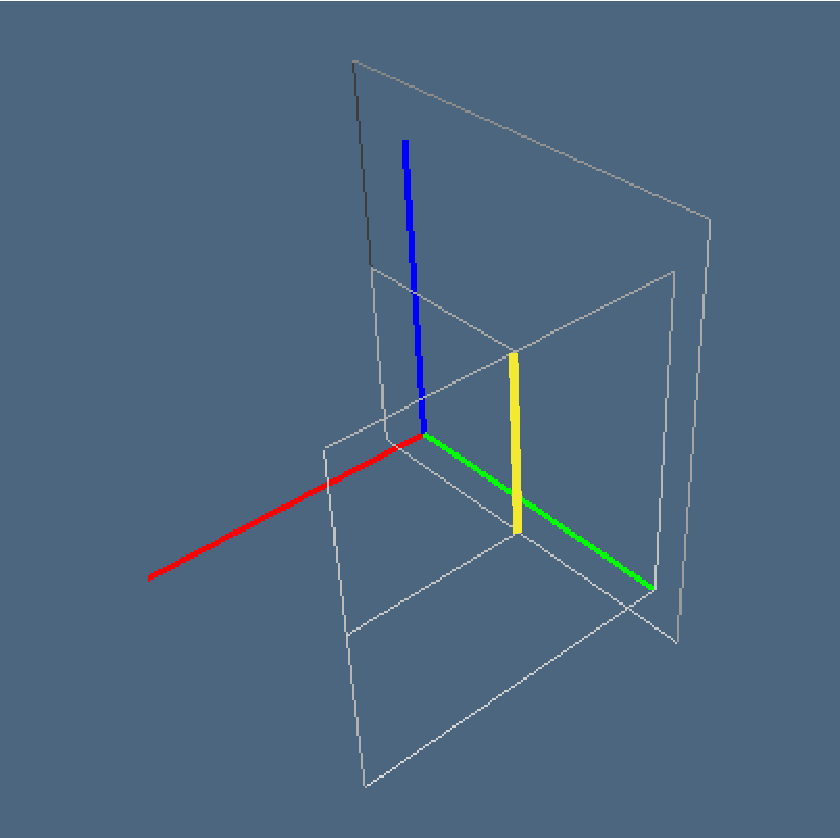
\includegraphics[height=0.325\linewidth,width=0.325\linewidth]{images/edgeTriangles1} 
   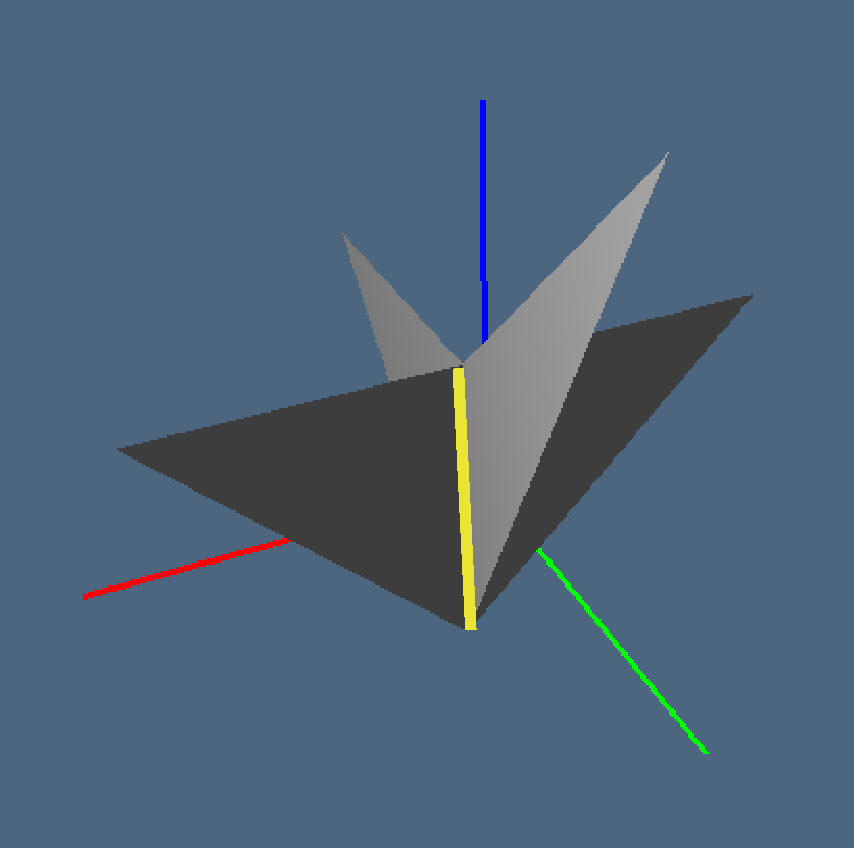
\includegraphics[height=0.325\linewidth,width=0.325\linewidth]{images/edgeTriangles} 
   \caption{The triangles around an edge: \texttt{VIEW(STRUCT(MKPOLS((W,ET[35]))))}.}
   \label{fig:3Dtriangulation}
\end{figure}

\paragraph{Example}

{\small
\begin{verbatim}
In [2]: ET[35]
Out[2]: [[19, 7, 8], [6, 8, 7], [8, 7, 16], [4, 7, 8]]

In [3]: EF[35]
Out[3]: [4, 10, 11, 14]

In [4]: [FW[f] for f in  EF[35]]
Out[4]: [(19, 7, 8, 12), (6, 10, 8, 7), (12, 8, 7, 16, 1, 2), (4, 5, 6, 7, 8, 9)]

In [5]: EW[35]
Out[5]: (7, 8)
\end{verbatim}}



\paragraph{Slope of edges}

The \texttt{faceSlopeOrdering} function, given in the script below, return the list \texttt{EF\_angle} of lists of faces incident to the model edges, counterclockwise ordered with respect to the orientation of the edge. Let us remember that the edges are naturally oriented from the vertex of lesser index to that of greater index.

%-------------------------------------------------------------------------------
@D Slope of edges
@{""" Circular ordering of faces around edges """

def planeProjection(normals):
    V = mat(normals)
    if all(V[:,0]==0): V = np.delete(V, 0, 1)
    elif all(V[:,1]==0): V = np.delete(V, 1, 1)
    elif all(V[:,2]==0): V = np.delete(V, 2, 1)
    return V

def faceSlopeOrdering(model,FE):
    V,FV,EV = model
    print "\nV",V
    print "\nFV",FV
    print "\nEV",EV
    print "\nFE",FE
    triangleSet = boundaryTriangulation(V,FV,EV,FE)
    TV = triangleIndices(triangleSet,V)
    triangleVertices = CAT(TV)
    TE = crossRelation(triangleVertices,EV)
    ET,ET_angle = invertRelation(TE),[]
    #import pdb; pdb.set_trace()
    for e,et in enumerate(ET):
        v1,v2 = EV[e]
        v1v2 = set([v1,v2])
        et_angle = []
        t0 = et[0]
        tverts = [v1,v2] + list(set(triangleVertices[t0]).difference(v1v2))
        e3 = UNITVECT(VECTDIFF([ V[tverts[1]], V[tverts[0]] ]))
        e1 = UNITVECT(VECTDIFF([ V[tverts[2]], V[tverts[0]] ]))
        e2 = cross(array(e1),e3).tolist()
        basis = mat([e1,e2,e3]).T
        transform = basis.I
        normals = []
        Tvs = []
        for triangle in et:
            verts = triangleVertices[triangle]
            vertSet = set(verts).difference(v1v2)
            tvs = [v1,v2] + list(vertSet)
            Tvs += [tvs]
            w1 = UNITVECT(VECTDIFF([ V[tvs[2]], V[tvs[0]] ]))
            w2 = (transform * mat([w1]).T).T
            w3 = cross(array([0,0,1]),w2).tolist()[0]
            normals += [w3]
        normals = mat(normals)
        for k,t in enumerate(et):
            angle = math.atan2(normals[k,1],normals[k,0])
            et_angle += [angle]
        pairs = sorted(zip(et_angle,et,Tvs))
        sortedTrias = [pair[1] for pair in pairs]
        triasVerts = [pair[2] for pair in pairs]
        tetraVerts = triasVerts[0]+[triasVerts[1][2]]
        ET_angle += [sortedTrias]
    EF_angle = ET_to_EF_incidence(TV,FV, ET_angle)
    return EF_angle
@}
%-------------------------------------------------------------------------------



\paragraph{Edge-triangles to Edge-faces incidence}

In the function \texttt{ET\_to\_EF\_incidence} below, we convert the Edge-triangles incidence table \texttt{ET\_angle} to a Edge-faces incidence table \texttt{EF\_angle}. The input data to the algoritm are the relations \texttt{TW,FW}, and, of course, the incidence \texttt{ET\_angle}. It works by computing two translationa tables \texttt{tableFT} and \texttt{tableTF} from face indices to triangle indices and viceversa. Of course, \texttt{assert( len(EF\_angle) == 2*len(FW) )} must be \texttt{True}.

%-------------------------------------------------------------------------------
@D Edge-triangles to Edge-faces incidence
@{""" Edge-triangles to Edge-faces incidence """
def ET_to_EF_incidence(TW,FW, ET_angle):
    tableFT = [None for k in range(len(FW))]
    t = 0
    for f,trias in enumerate(TW):
        tableFT[f] = range(t,t+len(trias))
        t += len(trias)
    tableTF = invertRelation(tableFT)
    EF_angle = [[tableTF[t][0] for t in triangles] for triangles in ET_angle]
    #assert( len(EF_angle) == 2*len(FW) )
    return EF_angle
@}
%-------------------------------------------------------------------------------


\paragraph{Cells from $(d-1)$-dimensional LAR model}
Since faces in the space partition induced by overlaping 3-coverings are $(d-1)$-cells, they are located on the boundary of \emph{two} $d$-cells of the partition. Hence, the traversal algorithm of the data structure storing the relevant information may be driven by signing the two cofaces of each face as being either already visited or not.


\subsection{Progressive reconstruction of 3-cell boundaries}

The input to this stage is a 2-complex embedded in 3D, with 2-cells non necessarily convex. The output is the 3-space partition defined by the cellular 3-complex, whose 2-skeleton is the inpiut complex. In other words, we mu reconstruct the 3-cells induced by the 2-cells of the input complex. This is done reconstructing the 3-cells stepwise. Each 3-cell reconstruction is done starting from one \texttt{face} two-dimensional previously taken into account no more than one single time, so that every 2-face is used at most exacly twice. An example of use of the functions implemented in this section is given in example \texttt{test12.py}

\paragraph{Edge cycles associated to a closed chain of edges}

The problem here is to conserve in the new \texttt{cycles} the same orientation of the previous ones,
passed through the \texttt{orientedEdges} variable. We can formalize the problem as follows. Let call \texttt{pcycles} (for ``previous cycles'') and \texttt{fcycle} (for ``face cycle'') the algorithm input. the output is the \emph{coherently oriented} \texttt{outcycles}. First, an orientation is given to \texttt{fcycle}; then this one is compared with the \texttt{pcycles} orientation, and it is possibly reversed, in order to get them coherently oriented. Finally, the direct sum of \texttt{pcycles} and \texttt{fcycle} is executed, giving the \texttt{outcycles}.

%-------------------------------------------------------------------------------
@D Cycles orientation
@{""" Cycles orientation """
def cyclesOrient(pcycles,fcycle,EV):
    if set(AA(ABS)(pcycles)).difference(fcycle)==set(): return []
    ofcycle = boundaryCycles(fcycle,EV)[0] # oriented 
    if type(pcycles[0])==list: opcycle = CAT(pcycles)
    else: opcycle = pcycles
    int = set(opcycle).intersection(ofcycle)
    if int != set(): 
        ofcycle = reverseOrientation(ofcycle)
    outChain = [e for e in ofcycle if not (-e in opcycle)] 
    outChain += [e for e in opcycle if not (-e in ofcycle)] 
    return outChain

if __name__ == "__main__":
    pcycles = [[-19, 13, 22, 23]]
    fcycle = [30, 20, 18, 2, 26, 19]
    #cyclesOrientation(pcycles,fcycle)
@}
%-------------------------------------------------------------------------------

%-------------------------------------------------------------------------------
@D Edge cycles associated to a closed chain of edges
@{""" Edge cycles associated to a closed chain of edges """
def boundaryCycles(edgeBoundary,EV):
    verts2edges = defaultdict(list)
    for e in edgeBoundary:
        verts2edges[EV[e][0]] += [e]
        verts2edges[EV[e][1]] += [e]
    cycles = []
    cbe = copy(edgeBoundary)
    while cbe != []:
        e = cbe[0]
        v = EV[e][0]
        cycle = []
        while True:
            cycle += [(e,v)]
            e = list(set(verts2edges[v]).difference([e]))[0]
            cbe.remove(e)
            v = list(set(EV[e]).difference([v]))[0]
            if (e,v)==cycle[0]:
                break
        n = len(cycle)
        cycles += [[e if EV[e]==(cycle[(k-1)%n][1],cycle[k%n][1]) else -e 
            for k,(e,v) in enumerate(cycle)]]
    return cycles
@}
%-------------------------------------------------------------------------------




\paragraph{The 3-cell traversal algorithm}
Initially, the list of counterclockwise ordered faces around the oriented edges are computed, and stored as indexed by edges in the \texttt{EF\_angle} list of lists. This information is stored in the compressed sparse row matrix \texttt{csrEF}, whose element $(e,f)$ provides the \emph{next} face index  incident on edge $e$, after $f$. 

Also, a list of list of zeros is stored in the \texttt{visitedFE} variable, in order to memorize the visited pairs $(f,e)$ by writing one in their corresponding positions. The \texttt{firstSearch} function will so retrieve the first non visited pair, in order to start the extraction of a new 3-cell. The \texttt{cv} variable accumulates the vertex indices of the current 3-cell. When the 3-cell is completely extracted (how-to test?), will be stored as a new row in the \texttt{CV} relation. 

The test for completeness of the extraction is done by computing the current boundary of the cell as a set of edges of faces, by python \texttt{XOR} of the edges of every accumulated face-edge relation. When this set it becomes empty, the 3-cell extraction is completed.
%-------------------------------------------------------------------------------
@D Cells from $(d-1)$-dimensional LAR model
@{""" Cells from $(d-1)$-dimensional LAR model """

def facesFromComponents(model,FE,EF_angle):
    # initialization
    V,FV,EV = model
    visitedCell = [[ None, None ] for k in range(len(FV)) ]
    face = 0
    boundaryLoop = boundaryCycles(FE[face],EV)[0]
    firstEdge = boundaryLoop[0]
    #import pdb; pdb.set_trace()
    cf,coe = getSolidCell(FE,face,visitedCell,boundaryLoop,EV,EF_angle,V,FV)
    for face,edge in zip(cf,coe):
        if visitedCell[face][0]==None: visitedCell[face][0] = edge
        else: visitedCell[face][1] = edge
    cv,ce = set(),set()
    cv = cv.union(CAT([FV[f] for f in cf]))
    ce = ce.union(CAT([FE[f] for f in cf]))
    CF,CV,CE,COE = [cf],[list(cv)],[list(ce)],[coe]
    
    # main loop
    while True:
        face, edge = startCell(visitedCell,FE,EV)
        if face == -1: break
        boundaryLoop = boundaryCycles(FE[face],EV)[0]
        if edge not in boundaryLoop:
            boundaryLoop = reverseOrientation(boundaryLoop)
        cf,coe = getSolidCell(FE,face,visitedCell,boundaryLoop,EV,EF_angle,V,FV)
        CF += [cf]
        COE += [coe]
        for face,edge in zip(cf,coe):
            if visitedCell[face][0]==None: visitedCell[face][0] = edge
            else: visitedCell[face][1] = edge
            
        cv,ce = set(),set()
        cv = cv.union(CAT([FV[f] for f in cf]))
        ce = ce.union(CAT([FE[f] for f in cf]))
        CV += [list(cv)]
        CE += [list(ce)]
    return V,CV,FV,EV,CF,CE,COE
@}
%-------------------------------------------------------------------------------
    

\paragraph{Start a new 3-cell}
The function \texttt{startCell} below is used to begin the extraction of a new 3-cell (after the first one was already extracted). Therefore its aim is to choose as first face one already previously extracted, in order to begin the current boundary with one cycle coherently oriented. This will is implemented by looking for a ``\texttt{face}'' position stored in \texttt{visitedCell} with just one \texttt{None} value in its row.

%-------------------------------------------------------------------------------
@D Start a new 3-cell
@{""" Start a new 3-cell """
def startCell(visitedCell,FE,EV):
    if len([term for cell in visitedCell for term in cell if term==None])==1: return -1,-1
    for face in range(len(visitedCell)):
        if len([term for term in visitedCell[face] if term==None])==1:
            edge = visitedCell[face][0]
            break
        else: pass  #TODO: implement search for isolated shells
        face,edge = -1,-1
    return face,edge
@}
%-------------------------------------------------------------------------------

\paragraph{Face orientations storage}

In order to correctly accomplish the extraction of 3-cells from the 2-complex partition of the arguments' space, it is necessary to use twice every 2-face, belonging with opposite orientations to the boundaries of two adjacent 3-cells. The array \texttt{faceOrientations}, initializated to $n\times 2$ zeros, with $n$ equal to the number of 2-cells, is so used to store the orientations of faces considered as 2-cycles of edges. 

In particular, the orientation of the 2-face is equivalent to the embedded orientation of one of its edges, corresponding either to the intrinsic orientation of this one, or to its opposite orientation. Hence, every time a face is used during the extraction of a 3-cell, (the elementary 1-chain of) one of its oriented edges is stored in \texttt{faceOrientations}, to remember its orientation, and eventually reverse the orientation of the face the next time it is used again. At the very end of the extraction algorithm, all the faces must be used twice, with opposite orientations. 

%-------------------------------------------------------------------------------
@D Face orientations storage
@{""" Face orientations storage """
def reverseOrientation(chain):
    return REVERSE([-cell for cell in chain])

def faceOrientation(boundaryLoop,face,FE,EV,cf):
    theBoundary = set(AA(ABS)(boundaryLoop))
    if theBoundary.intersection(FE[face])==set() and theBoundary.difference(FE[face])!=set(): ##BOH!!
        coboundaryFaces = [f for f in cf if set(FE[f]).intersection(theBoundary)!=set()]
        face = coboundaryFaces[0]            
    faceLoop = boundaryCycles(FE[face],EV)[0]
    commonEdges = set(faceLoop).intersection(boundaryLoop)
    if commonEdges == set() or commonEdges == {0}: 
        faceLoop = reverseOrientation(faceLoop)
        commonEdges = set(faceLoop).intersection(boundaryLoop)
    theEdge = list(commonEdges)[0]
    #if theEdge==0: theEdge = list(commonEdges)[1]
    return -theEdge,face
@}
%-------------------------------------------------------------------------------

\paragraph{Get single solid cell}

%-------------------------------------------------------------------------------
@D Get single solid cell
@{""" Get single solid cell """
def getSolidCell(FE,face,visitedCell,boundaryLoop,EV,EF_angle,V,FV):

    def orientFace(face,boundaryLoop): 
        for e in boundaryLoop:
            if ABS(e) in FE[face]: return -e

    coe = [orientFace(face,boundaryLoop)]
    cf = [face] 
    while boundaryLoop != []:
        edge,face = faceOrientation(boundaryLoop,face,FE,EV,cf)
        if edge > 0: edgeFaces = EF_angle[edge]
        elif edge < 0: edgeFaces = REVERSE(EF_angle[-edge])
        e = ABS(edge)
        n = len(edgeFaces)
        ind = (edgeFaces.index(face)+1)%n
        nextFace = edgeFaces[ind]
        coe += [-orientFace(nextFace,boundaryLoop)]
        boundaryLoop = cyclesOrient(boundaryLoop,FE[nextFace],EV)
        cf += [nextFace] 
        face = nextFace
    if DEBUG: pass
        #VIEW(EXPLODE(1.2,1.2,1.2)( MKTRIANGLES(V,[FV[f] for f in cf]) ))
    return cf,coe
@}
%-------------------------------------------------------------------------------

\paragraph{Double check the faces boundaries made of edges}
Let us notice that a sistematic use of the \texttt{FE} relation to compute the edges on the boundary of a face is \emph{not} reliable when the faces are non-convex. A better solution is to double-check the result \texttt{FE[f]} when \texttt{len(FE[f]) > len(FV[f])}, in order to filter out the spurious edges ...
The function below works with the precondition that vertices in \texttt{FV[f]} are spatially ordered along the face boundary.

%-------------------------------------------------------------------------------
@D Double check the faces boundaries made of edges
@{""" Double check the faces boundaries made of edges """
def doubleCheckFaceBoundaries(FE,V,FV,EV):
    FEout = []
    for f,face in enumerate(FE):
        n = len(FV[f])
        if len(FE[f]) > n:
            verts = list(FV[f])+[FV[f][0]]
            edges = [sorted([verts[k],verts[k+1]]) for k in range(n)]
            edgeDict = dict()
            for e in FE[f]: edgeDict[EV[e]] = e
            orderedEdges = [edgeDict[tuple(edge)] for edge in edges]
            assert len(orderedEdges)==len(verts)-1
            FEout += [orderedEdges]
        else:
            FEout += [face]
    return FEout
@}
%-------------------------------------------------------------------------------


\subsubsection{Main procedure of arrangement partitioning}

%-------------------------------------------------------------------------------
@D Main procedure of arrangement partitioning
@{""" Main procedure of arrangement partitioning """

@< Double check the faces boundaries made of edges @>

def thePartition(W,FW,EW):
    quadArray = [[W[v] for v in face] for face in FW]
    parts = boxBuckets(containmentBoxes(quadArray))

    #import pdb; pdb.set_trace()
    Z,FZ,EZ = spacePartition(W,FW,EW, parts)
    print "Z =",Z
    print "FZ =",FZ
    print "EZ =",EZ
    
    EZ = [EZ[0]]+EZ
    model = Z,FZ,EZ

    ZZ = AA(LIST)(range(len(Z)))
    submodel = STRUCT(MKPOLS((Z,EZ)))
    VIEW(larModelNumbering(1,1,1)(Z,[ZZ,EZ,FZ],submodel,0.4)) 
    #import pdb; pdb.set_trace()

    FE = crossRelation(FZ,EZ) ## to be double checked !!
    FE = doubleCheckFaceBoundaries(FE,Z,FZ,EZ)
    
    # remove 0 indices from FE relation
    FE = [[f if f!=0 else 1 for f in face] for face in FE]
    EF_angle = faceSlopeOrdering(model,FE)
    
    V,CV,FV,EV,CF,CE,COE = facesFromComponents((Z,FZ,EZ),FE,EF_angle)
    return V,CV,FV,EV,CF,CE,COE,FE
@}
%-------------------------------------------------------------------------------




\subsection{Boolean chains}
%===============================================================================

%===============================================================================
\section{Esporting the Library}
%===============================================================================

%-------------------------------------------------------------------------------
@O larlib/larlib/bool.py
@{""" Module for Boolean computations between geometric objects """
from larlib import *
DEBUG = False

@< Coding utilities @>
@< Split the boxes between the below,above subsets @>
@< Test if bucket OK or append to splitting stack @>
@< Remove subsets from bucket list @>
@< Iterate the splitting until splittingStack is empty @>
@< Computation of face transformations @>
@< Computation of affine face transformations @>
@< Computation of topological relation @>
@< Submanifold mapping computation @>
@< Set of line segments partitioning a facet @>
@< Check for superimposing edges @>
@< Space partitioning via submanifold mapping @>
@< Point in polygon testing @>
@< 3D boundary triangulation of the space partition @>
@< Computation of incidence between edges and 3D triangles @>
@< Directional and orthogonal projection operators @>
@< Check edge-face ordering @>
@< Slope of edges @>
@< Oriented cycle of vertices from a 1-cycle of unoriented edges @>
@< Edge-triangles to Edge-faces incidence @>
@< Cells from $(d-1)$-dimensional LAR model @>
@< Edge cycles associated to a closed chain of edges @>
@< Permutation of edges defined by edge cycles @>
@< Cycles orientation @>
@< Start a new 3-cell @>
@< Face orientations storage @>
@< Check and store the orientation of faces @>
@< Get single solid cell @>
@< Main procedure of arrangement partitioning @>
@}
%-------------------------------------------------------------------------------
    
%===============================================================================
\section{Test examples}
%===============================================================================

\subsection{Random triangles}
%===============================================================================


\paragraph{Generation of random triangles and their boxes}
%-------------------------------------------------------------------------------
@O test/py/bool/test01.py
@{""" Generation of random triangles and their boxes """
from larlib import *
glass = MATERIAL([1,0,0,0.1,  0,1,0,0.1,  0,0,1,0.1, 0,0,0,0.1, 100])

randomTriaArray = randomTriangles(10,0.99)
VIEW(STRUCT(AA(MKPOL)([[verts, [[1,2,3]], None] for verts in randomTriaArray])))

boxes = containmentBoxes(randomTriaArray)
hexas = AA(box2exa)(boxes)
cyan = COLOR(CYAN)(STRUCT(AA(MKPOL)([[verts, [[1,2,3]], None] for verts in randomTriaArray])))
yellow = STRUCT(AA(glass)(AA(MKPOL)([hex for hex,qualifier in hexas])))
VIEW(STRUCT([cyan,yellow]))
@}
%-------------------------------------------------------------------------------


\paragraph{Generation of random quadrilaterals and their boxes}
%-------------------------------------------------------------------------------
@O test/py/bool/test02.py
@{""" Generation of random quadrilaterals and their boxes """
from larlib import *
glass = MATERIAL([1,0,0,0.1,  0,1,0,0.1,  0,0,1,0.1, 0,0,0,0.1, 100])

randomQuadArray = randomQuads(10,1)
VIEW(STRUCT(AA(MKPOL)([[verts, [[1,2,3,4]], None] for verts in randomQuadArray])))

boxes = containmentBoxes(randomQuadArray)
hexas = AA(box2exa)(boxes)
cyan = COLOR(CYAN)(STRUCT(AA(MKPOL)([[verts, [[1,2,3,4]], None] for verts in randomQuadArray])))
yellow = STRUCT(AA(glass)(AA(MKPOL)([hex for hex,qualifier in hexas])))
VIEW(STRUCT([cyan,yellow]))
@}
%-------------------------------------------------------------------------------

\begin{figure}[htbp] %  figure placement: here, top, bottom, or page
   \centering
   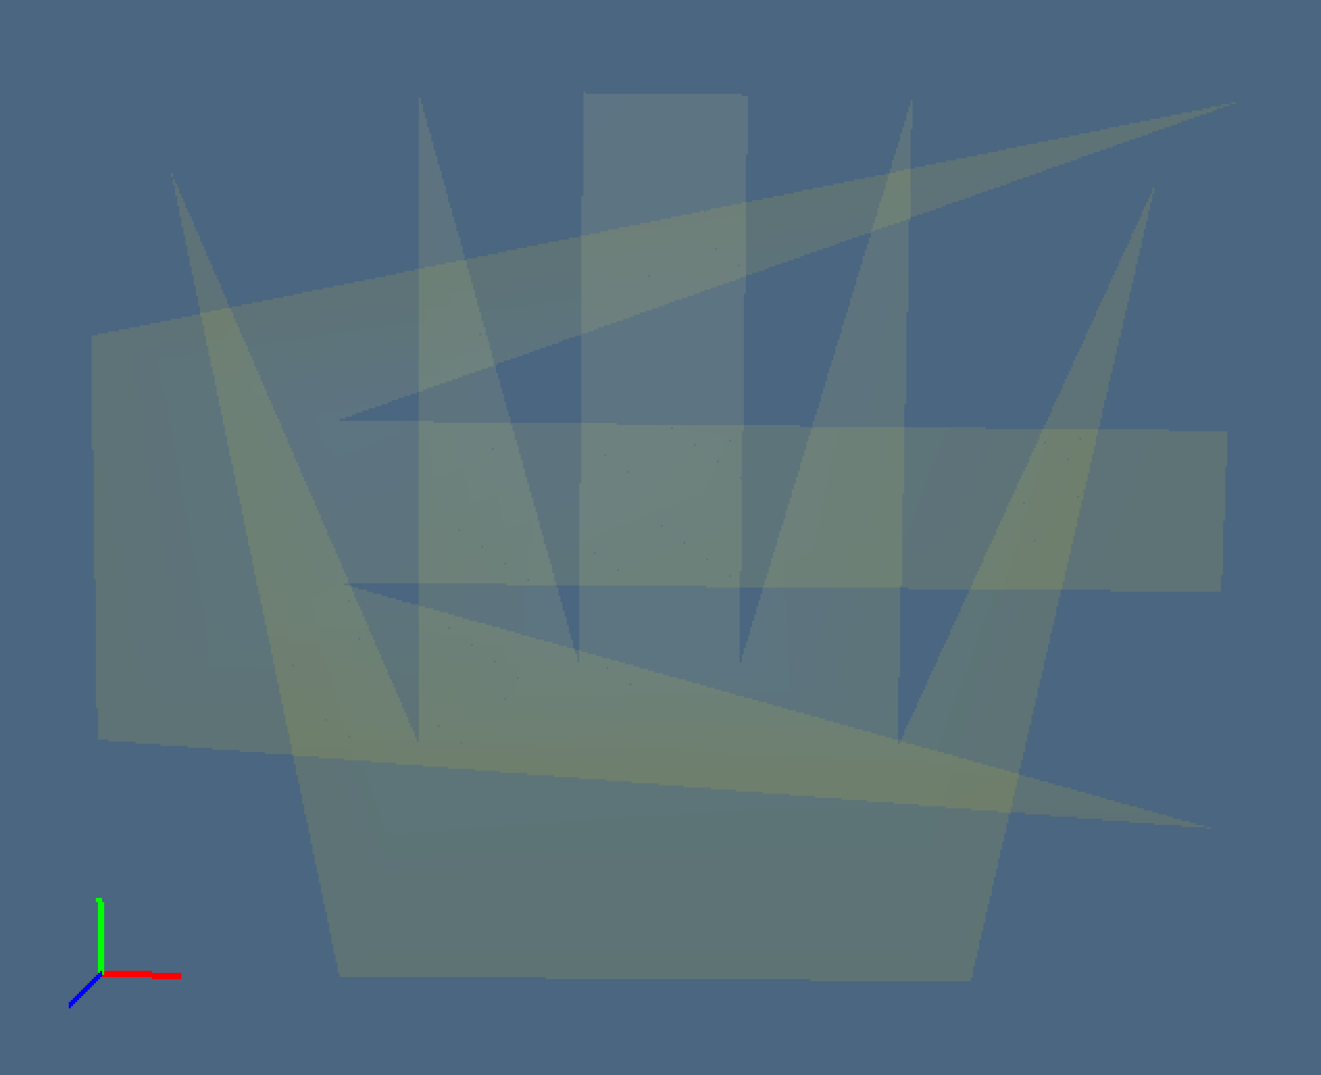
\includegraphics[height=0.2\linewidth,width=0.2425\linewidth]{images/fork1} 
   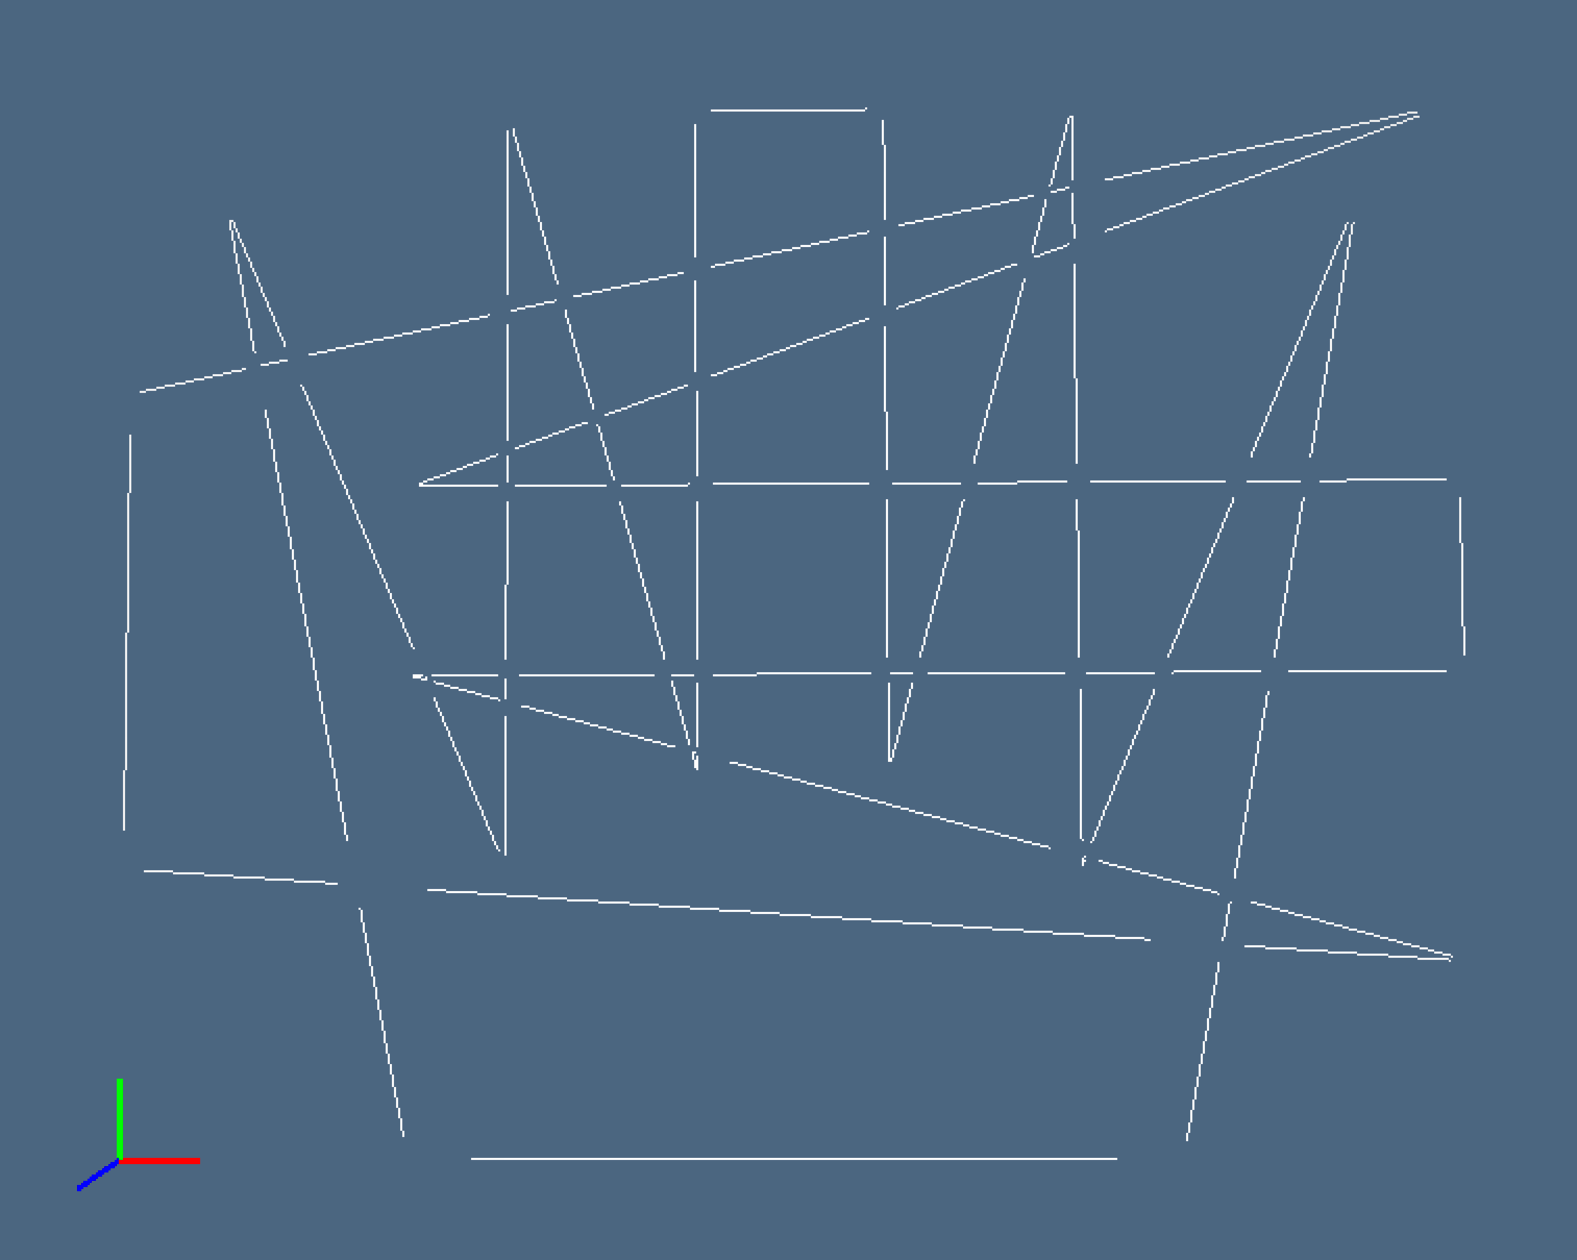
\includegraphics[height=0.2\linewidth,width=0.2425\linewidth]{images/fork2} 
   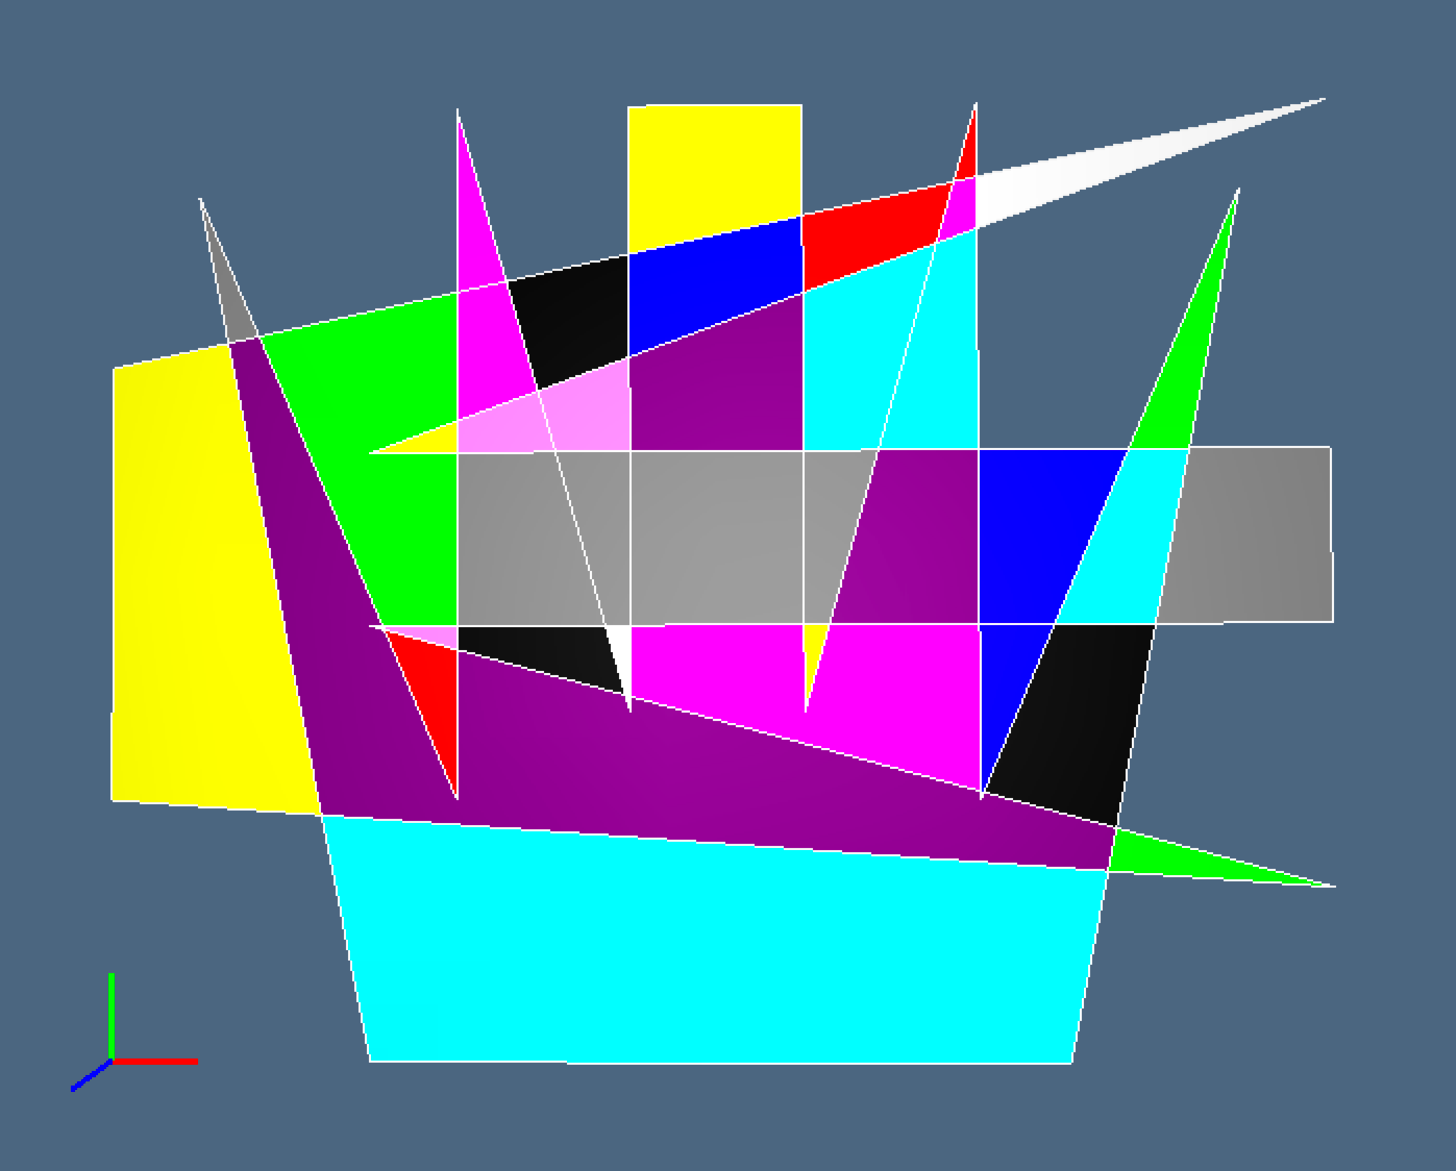
\includegraphics[height=0.2\linewidth,width=0.2425\linewidth]{images/fork3} 
   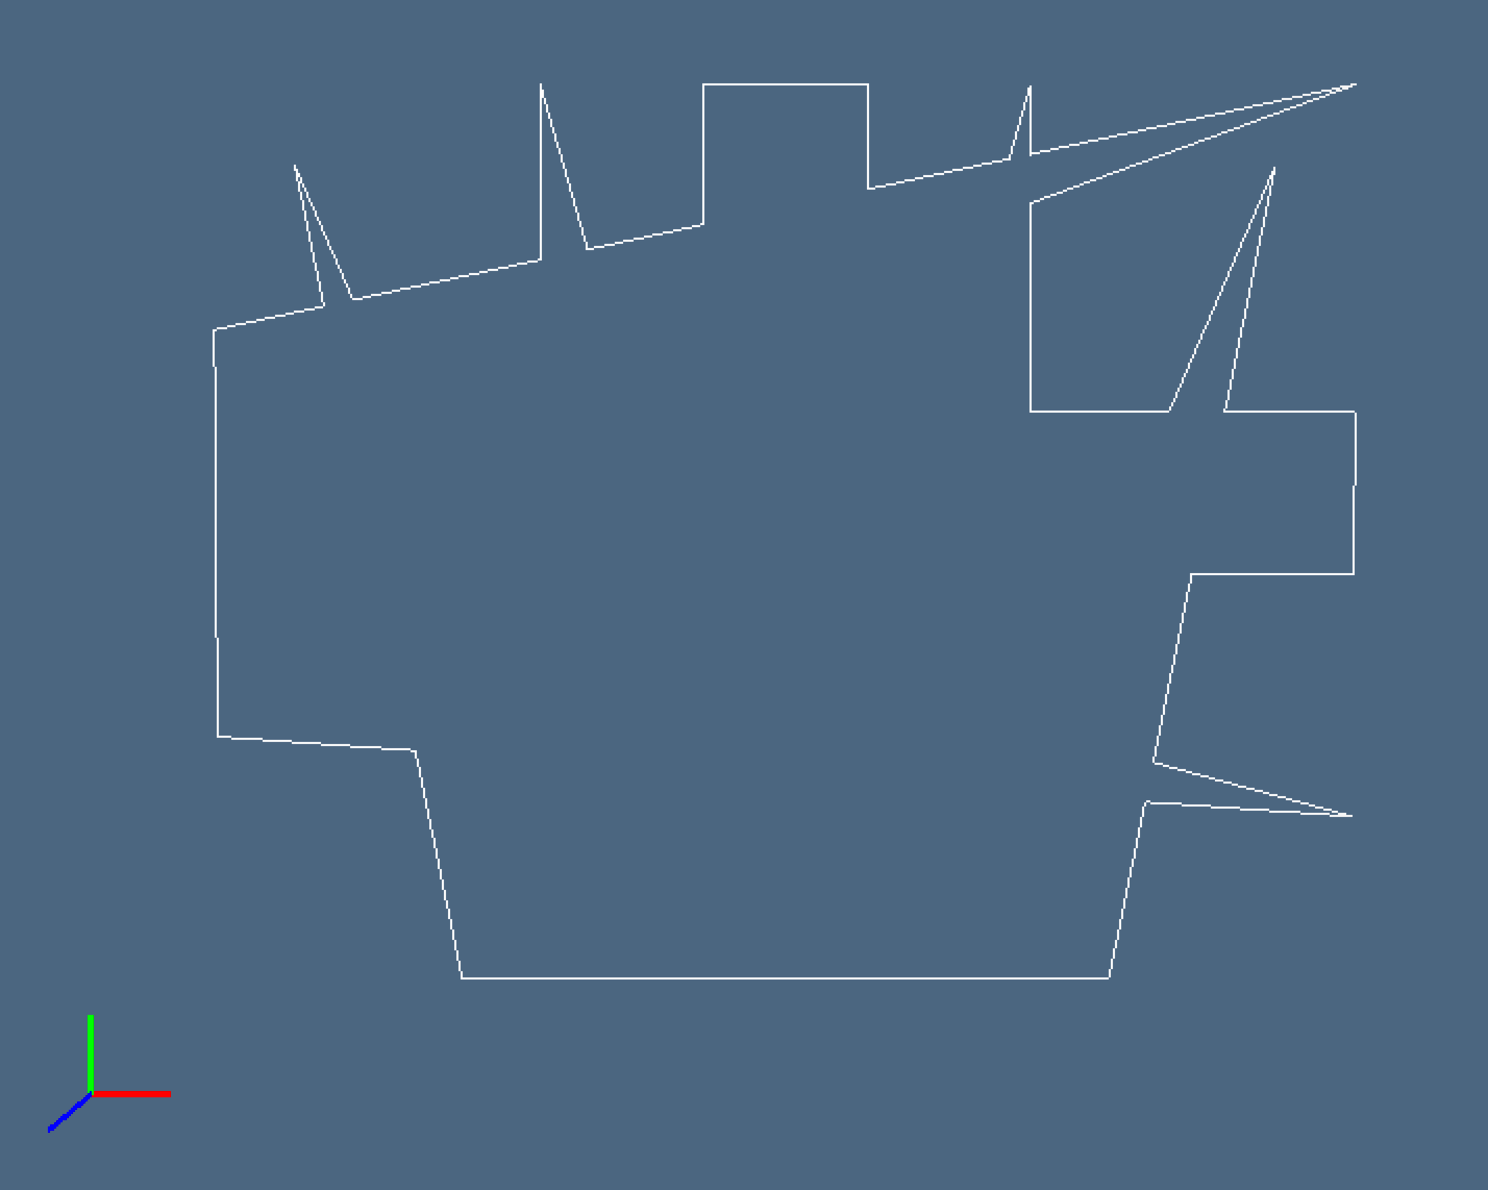
\includegraphics[height=0.2\linewidth,width=0.2425\linewidth]{images/fork4} 
   \caption{\texttt{LAR} complex from two polygons. (a) the input polygons; (b) the intersection of boundary lines; (c) the extracted \emph{regularized} 2-complex; (d) the boundary \texttt{LAR}.}
   \label{fig:ortho}
\end{figure}

%-------------------------------------------------------------------------------
@O test/py/bool/test03.py
@{""" Boolean complex generated by boundaries of two complexes """
from larlib import *
glass = MATERIAL([1,0,0,0.1,  0,1,0,0.1,  0,0,1,0.1, 0,0,0,0.1, 100])

V1 = [[3,0],[11,0],[13,10],[10,11],[8,11],[6,11],[4,11],[1,10],[4,3],[6,4],
        [8,4],[10,3]]
FV1 = [[0,1,8,9,10,11],[1,2,11],[3,10,11],[4,5,9,10],[6,8,9],[0,7,8]]
EV1 = [[0,1],[0,7],[0,8],[1,2],[1,11],[2,11],[3,10],[3,11],[4,5],[4,10],[5,
        9],[6,8],[6,9],[7,8],[8,9],[9,10],[10,11]]
BE1 = boundaryCells(FV1,EV1)
lines1 = [[V1[v] for v in EV1[edge]] for edge in BE1]

V2 = [[0,3],[14,2],[14,5],[14,7],[14,11],[0,8],[3,7],[3,5]]
FV2 = [[0,5,6,7],[0,1,7],[4,5,6],[2,3,6,7]]
EV2 = [[0,1],[0,5],[0,7],[1,7],[2,3],[2,7],[3,6],[4,5],[4,6],[5,6],[6,7]]
BE2 = boundaryCells(FV2,EV2)
lines2 = [[V2[v] for v in EV2[edge]] for edge in BE2]

VIEW(STRUCT([ glass(STRUCT(MKPOLS((V1,FV1)))), glass(STRUCT(MKPOLS((V2,FV2)))) ]))
lines = lines1 + lines2
VIEW(STRUCT(AA(POLYLINE)(lines)))

global precision
PRECISION -= 2
V,FV,EV = larFromLines(lines)
VIEW(EXPLODE(1.2,1.2,1)(MKPOLS((V,EV))))

VV = AA(LIST)(range(len(V)))
submodel = STRUCT(MKPOLS((V,EV)))
VIEW(larModelNumbering(1,1,1)(V,[VV,EV,FV[:-1]],submodel,1))

polylines = [[V[v] for v in face+[face[0]]] for face in FV[:-1]]
colors = [CYAN, MAGENTA, WHITE, RED, YELLOW, GREEN, GRAY, ORANGE, BLACK, BLUE, PURPLE, BROWN]
sets = [COLOR(colors[k%12])(FAN(pol)) for k,pol in enumerate(polylines)]
VIEW(STRUCT([ T(3)(0.02)(STRUCT(AA(POLYLINE)(lines))), STRUCT(sets)]))

VIEW(EXPLODE(1.2,1.2,1)((AA(POLYLINE)(polylines))))
polylines = [ [V[v] for v in FV[-1]+[FV[-1][0]]] ]
VIEW(EXPLODE(1.2,1.2,1)((AA(POLYLINE)(polylines))))
@}
%-------------------------------------------------------------------------------



\subsection{Testing the box-kd-trees}
%===============================================================================


\paragraph{Visualizing with different colors the buckets of box-kd-tree}
%-------------------------------------------------------------------------------
@O test/py/bool/test04.py @{
""" Visualizing with different colors the buckets of box-kd-tree """
from larlib import *

randomQuadArray = randomQuads(30,0.8)
VIEW(STRUCT(AA(MKPOL)([[verts, [[1,2,3,4]], None] for verts in randomQuadArray])))


V,[VV,EV,FV,CV] = larCuboids([2,2,1],True)
cubeGrid = Struct([(V,FV,EV)],"cubeGrid")
cubeGrids = Struct(2*[cubeGrid,s(.5,.5,.5)])
V,FV,EV = struct2lar(cubeGrids)
boxes = containmentBoxes([[V[v] for v in f] for f in FV])
VV = AA(LIST)(range(len(V)))
submodel = STRUCT(MKPOLS((V,EV)))
VIEW(larModelNumbering(1,1,1)(V,[VV,EV,FV],submodel,0.6)) 
parts = boxBuckets(boxes)
V,FV,EV = spacePartition(V,FV,EV, parts)
VV = AA(LIST)(range(len(V)))
submodel = STRUCT(MKPOLS((V,EV)))
VIEW(larModelNumbering(1,1,1)(V,[VV,EV,FV],submodel,0.6)) 


#boxes = containmentBoxes(randomQuadArray)
hexas = AA(box2exa)(boxes)
glass = MATERIAL([1,0,0,0.1,  0,1,0,0.1,  0,0,1,0.1, 0,0,0,0.1, 100])
yellow = STRUCT(AA(glass)(AA(MKPOL)([hex for hex,data in hexas])))
VIEW(STRUCT([#cyan,
    yellow]))

parts = boxBuckets(boxes)
for k,part in enumerate(parts):
    bunch = [glass(STRUCT( [MKPOL(hexas[h][0]) for h in part]))]
    bunch += [COLOR(RED)(MKPOL(hexas[k][0]))]
    if k==30: VIEW(STRUCT(bunch))
@}
%-------------------------------------------------------------------------------


\subsection{Intersection of geometry subsets}
%===============================================================================




\paragraph{Two unit cubes}
%-------------------------------------------------------------------------------
@D Two unit cubes 
@{""" Two unit cubes """
from larlib import *
V,[VV,EV,FV,CV] = larCuboids([1,1,1],True)
cube1 = Struct([(V,FV,EV)],"cube1")
twoCubes = Struct([cube1,t(.5,.5,.5),cube1])

glass = MATERIAL([1,0,0,0.1,  0,1,0,0.1,  0,0,1,0.1, 0,0,0,0.1, 100])

#twoCubes = Struct([cube1,t(-1,.5,1),cube1])     # other test example
#twoCubes = Struct([cube1,t(.5,.5,0),cube1])    # other test example
#twoCubes = Struct([cube1,t(.5,0,0),cube1])        # other test example

V,FV,EV = struct2lar(twoCubes)
VIEW(EXPLODE(1.2,1.2,1.2)(MKPOLS((V,FV))))

quadArray = [[V[v] for v in face] for face in FV]
boxes = containmentBoxes(quadArray)
hexas = AA(box2exa)(boxes)
parts = boxBuckets(boxes)
@}
%-------------------------------------------------------------------------------


def POLYGONS((V,FV)):



\begin{figure}[htbp] %  figure placement: here, top, bottom, or page
   \centering
   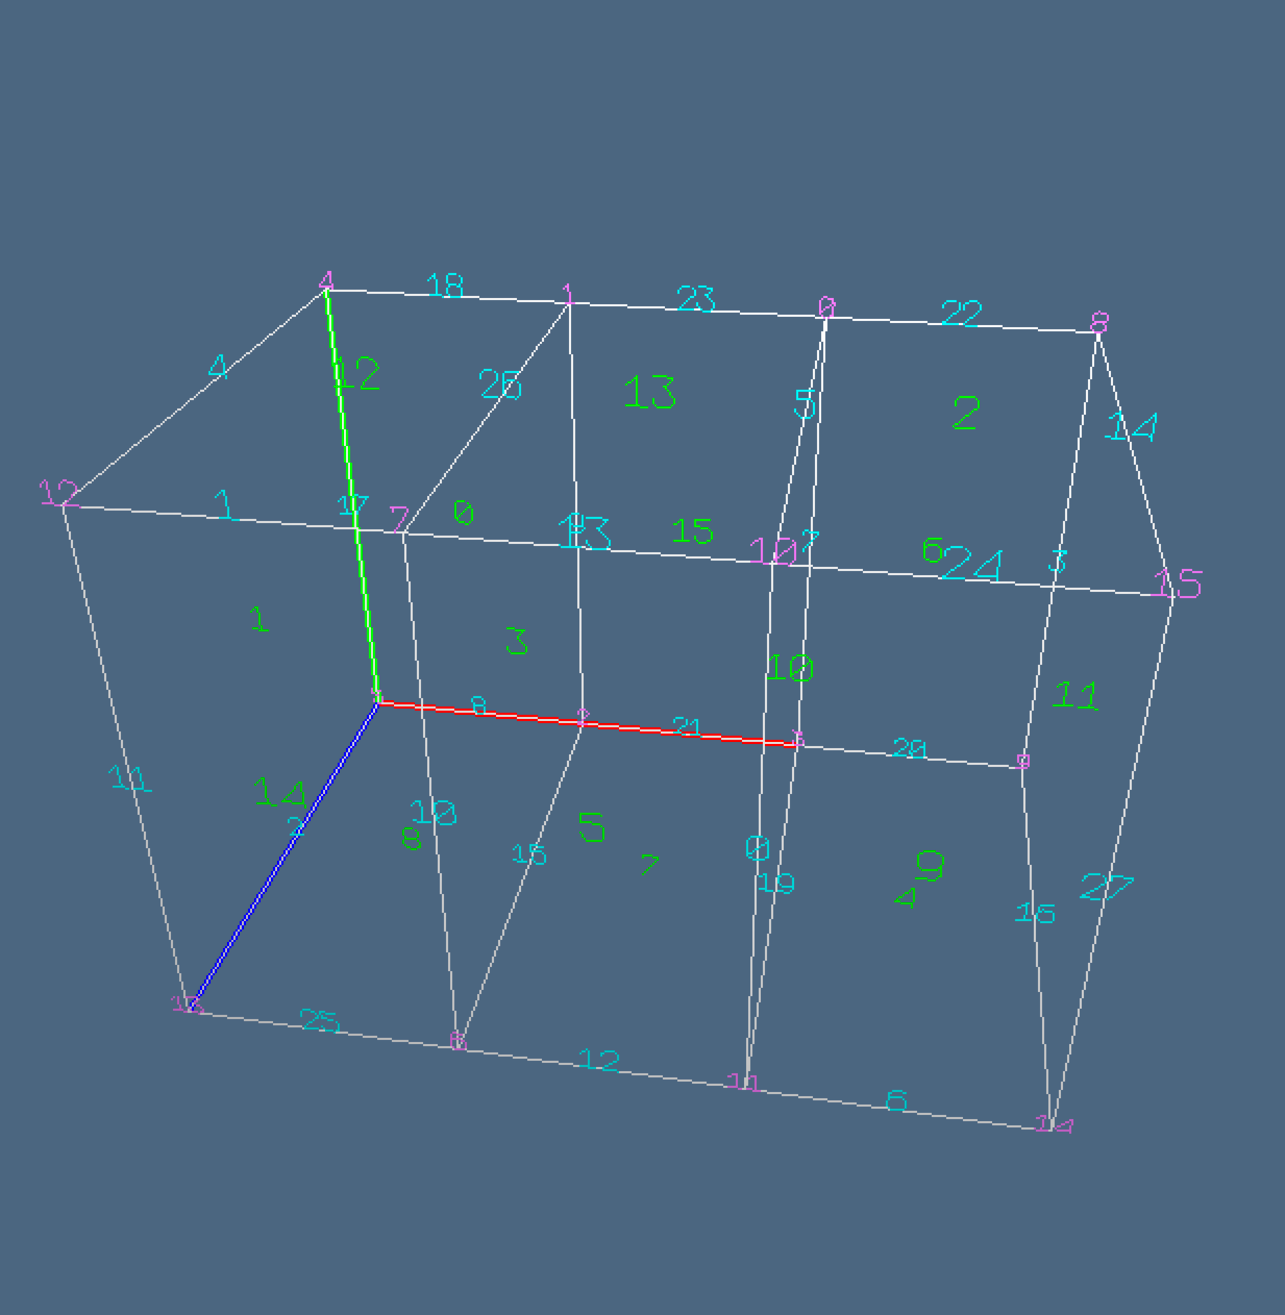
\includegraphics[height=0.245\linewidth,width=0.243\linewidth]{images/twocubes1} 
   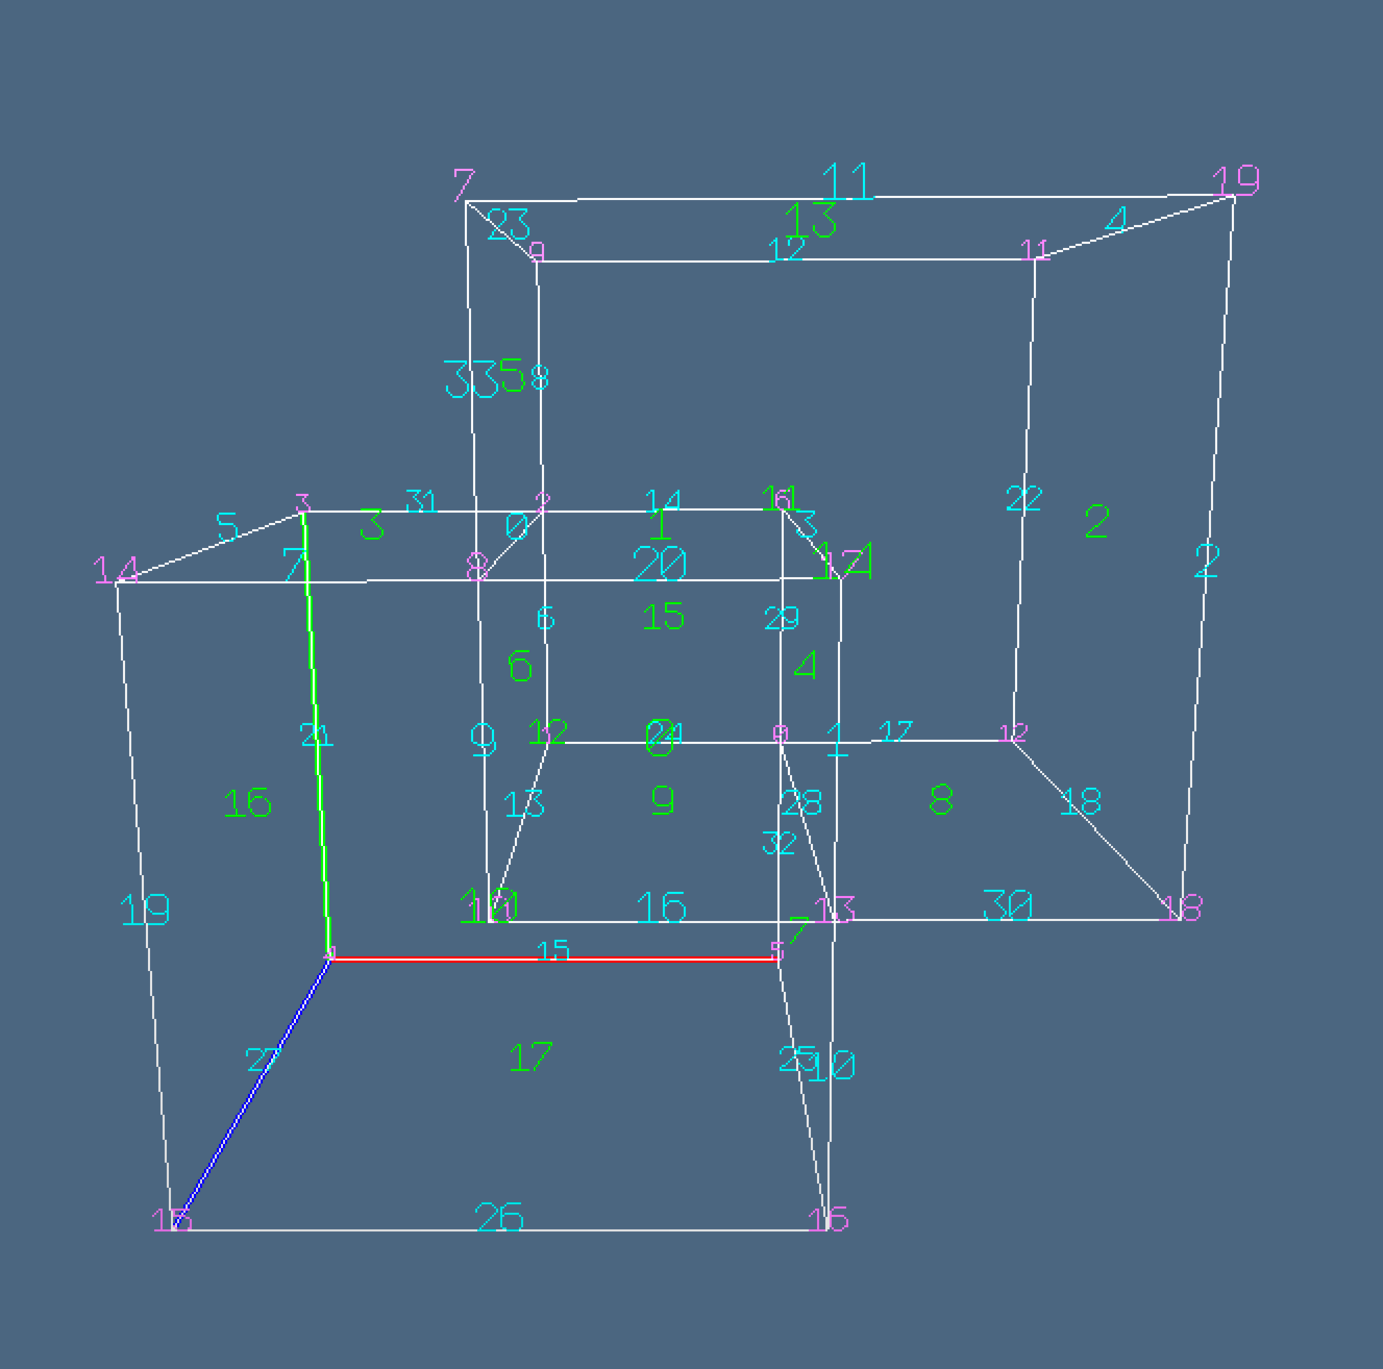
\includegraphics[height=0.245\linewidth,width=0.243\linewidth]{images/twocubes2} 
   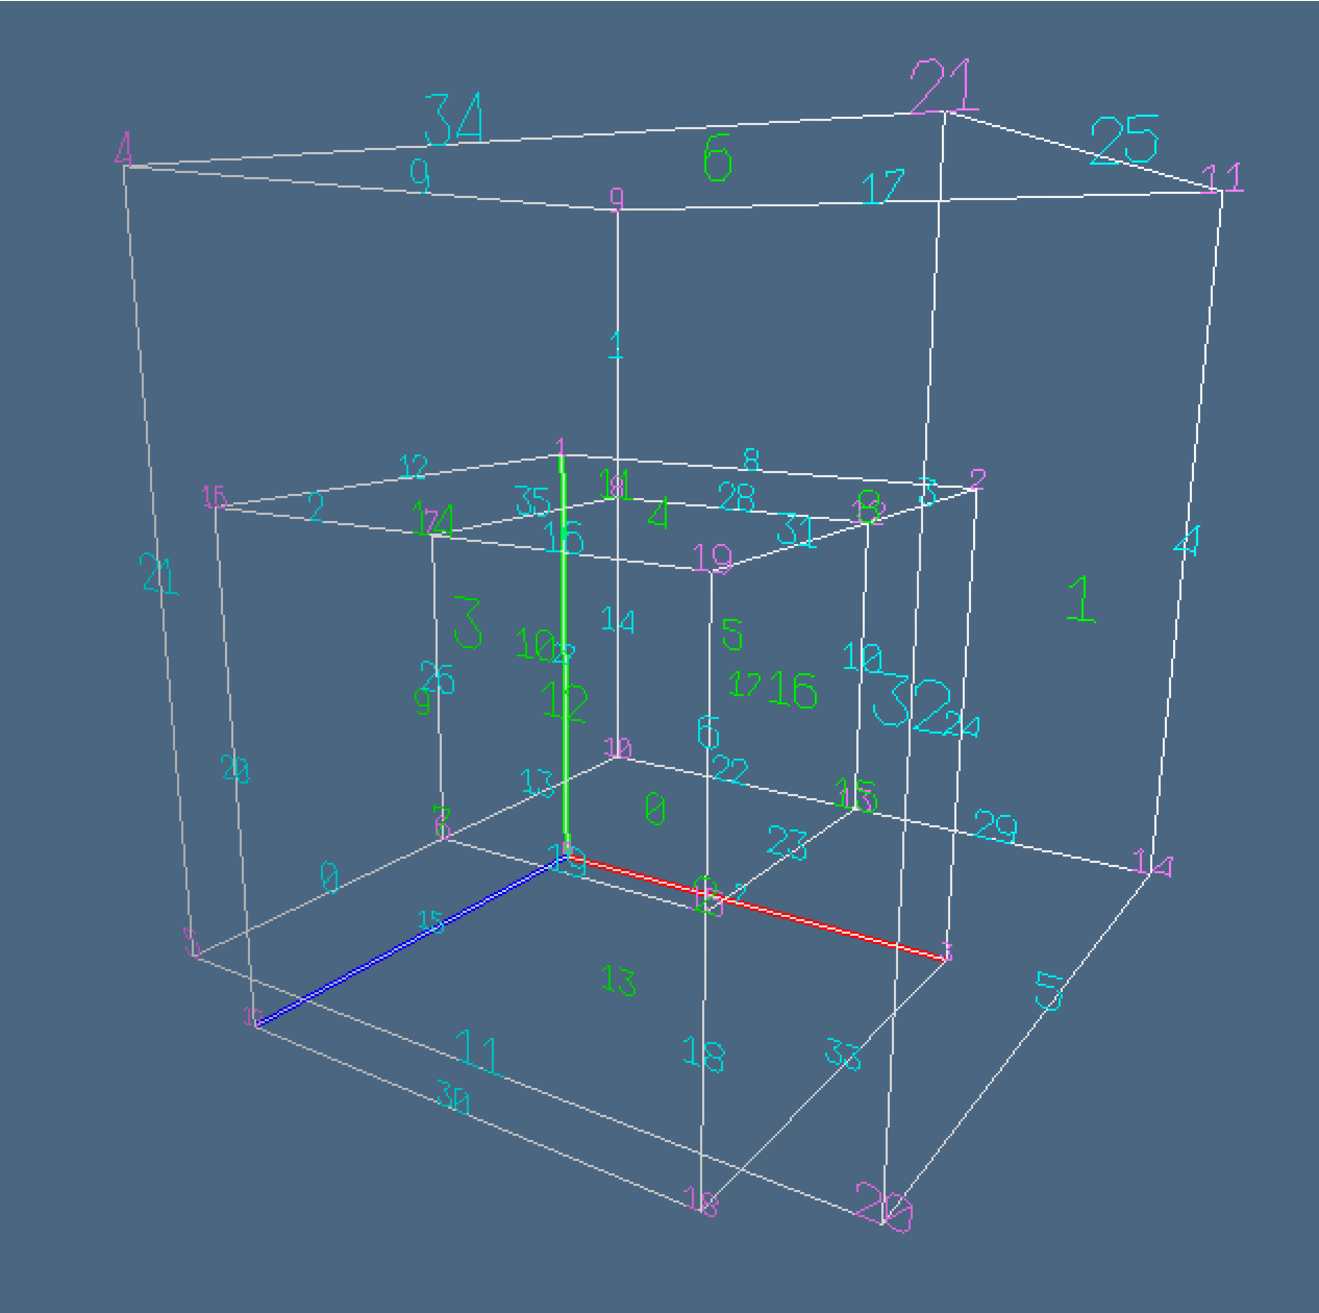
\includegraphics[height=0.245\linewidth,width=0.243\linewidth]{images/twocubes3} 
   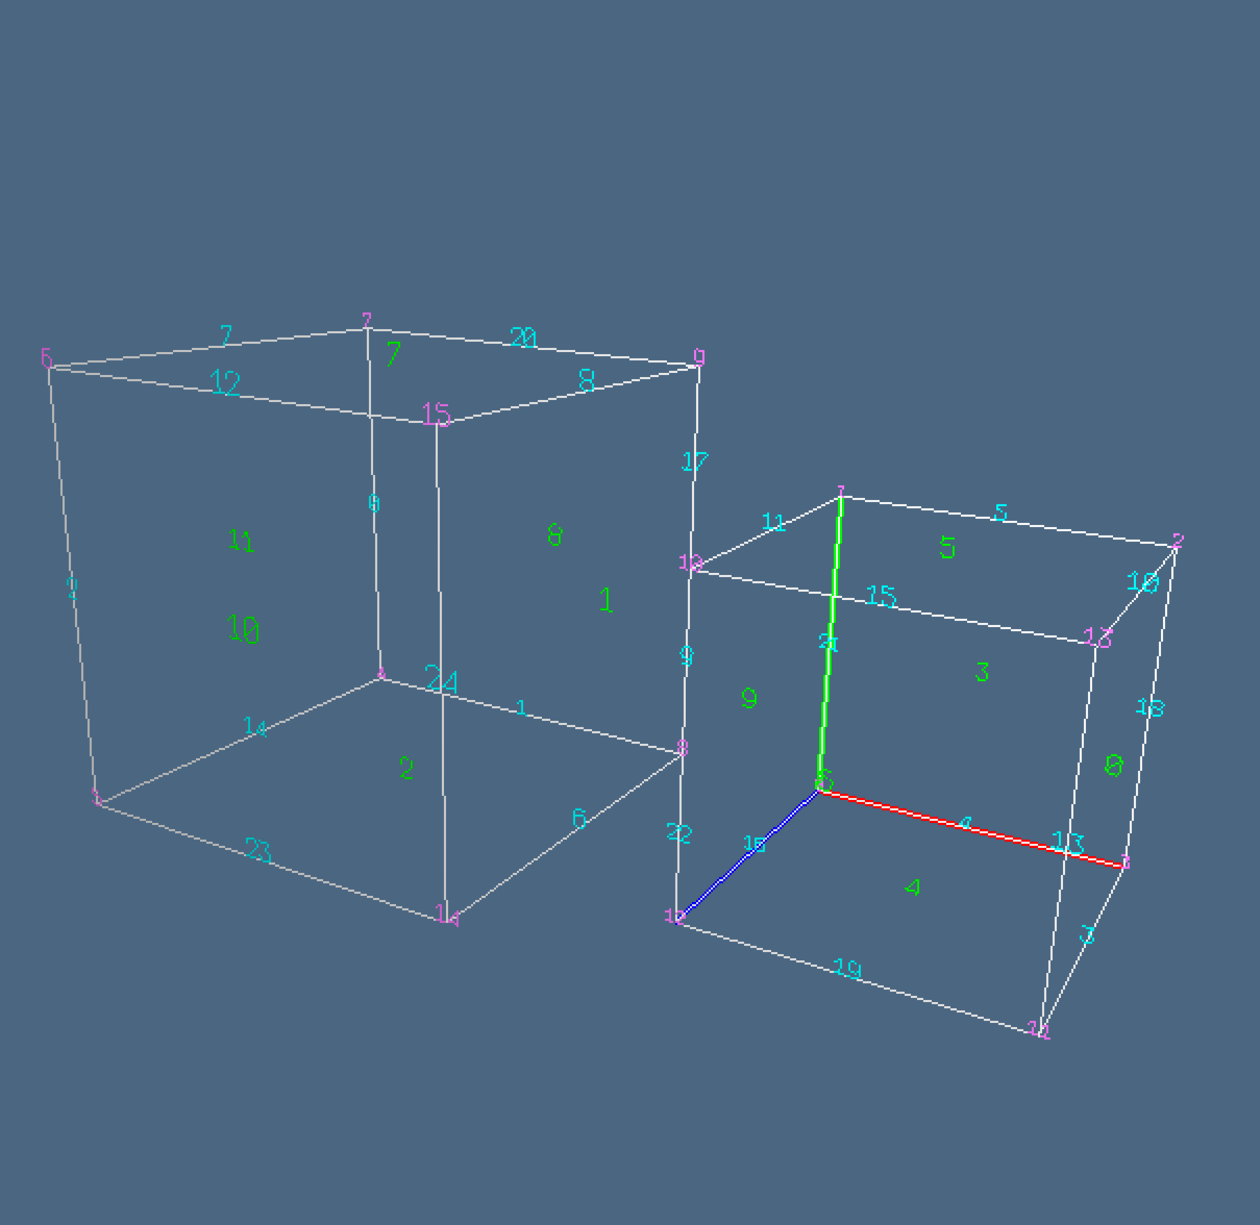
\includegraphics[height=0.245\linewidth,width=0.243\linewidth]{images/twocubes4} 
   \caption{\texttt{LAR} complex of the space decomposition generated by two cubes in special positions. (a) translation on one coordinate; (b) translation on two coordinates;  (c) translation on three coordinates; (d) non-manifold position along an edge.}
   \label{fig:twocubes}
\end{figure}


\paragraph{Face (and incident faces) transformation}
%-------------------------------------------------------------------------------
@O test/py/bool/test05.py
@{""" non-valid -> valid solid representation of a space partition """
from larlib import *

@< Two unit cubes @>
    
W,FW,EW = spacePartition(V,FV,EV, parts)
polylines = lar2polylines((W,FW))
VIEW(EXPLODE(1.2,1.2,1.2)(AA(POLYLINE)(polylines)))

WW = AA(LIST)(range(len(W)))
submodel = STRUCT(MKPOLS((W,EW)))
VIEW(larModelNumbering(1,1,1)(W,[WW,EW,FW],submodel,0.5))
@}
%-------------------------------------------------------------------------------







\paragraph{3-cell reconstruction from LAR space partition}
%-------------------------------------------------------------------------------
@O test/py/bool/test06.py
@{""" 3-cell reconstruction from LAR space partition """
from larlib import *
@< Two unit cubes @>
W,FW,EW = spacePartition(V,FV,EV, parts)
WW = AA(LIST)(range(len(W)))
submodel = STRUCT(MKPOLS((W,EW)))
VIEW(larModelNumbering(1,1,1)(W,[WW,EW,FW],submodel,0.6))
@}
%-------------------------------------------------------------------------------



\paragraph{2D polygon triangulation}
Here a 2D polygon is imported from an SVG file made of boundary lines, and the \texttt{V,FV,EV}
LAR model is generated. Then the unique polygonal face in \texttt{FV} is embedded in 3D ($z=0$), and triangulated using the tassellation algorithm extracted from pyOpenGL and pyGLContext, stored in the \texttt{lib/py/support.py} file. The generated triangles are finally coherently oriented, by testing the $z$-component of their normal vector.

%-------------------------------------------------------------------------------
@O test/py/bool/test07.py
@{""" 2D polygon triangulation """
from larlib import *

filename = "test/svg/bool/interior.svg"
lines = svg2lines(filename)    
V,FV,EV = larFromLines(lines)
VIEW(EXPLODE(1.2,1.2,1)(MKPOLS((V,FV[:-1]+EV)) + AA(MK)(V)))

pivotFace = [V[v] for v in FV[0]+[FV[0][0]]]
pol = PolygonTessellator()
vertices = [ vertex.Vertex( (x,y,0) ) for (x,y) in pivotFace  ]
verts = pol.tessellate(vertices)
ps = [list(v.point) for v in verts]
trias = [[ps[k],ps[k+1],ps[k+2],ps[k]] for k in range(0,len(ps),3)]
VIEW(STRUCT(AA(POLYLINE)(trias)))

triangles = DISTR([AA(orientTriangle)(trias),[[0,1,2]]])
VIEW(STRUCT(CAT(AA(MKPOLS)(triangles))))
@}
%-------------------------------------------------------------------------------


\paragraph{From triples of points to LAR model of boundary triangulation}
    
%-------------------------------------------------------------------------------
@O test/py/bool/test08.py @{
import sys
from larlib import *

sys.path.insert(0, 'test/py/bool/')
from test06 import *

""" From triples of points to LAR model """
FE = crossRelation(FW,EW)
triangleSet = boundaryTriangulation(W,FW,EW,FE)
TW = triangleIndices(triangleSet,W)
VIEW(EXPLODE(1.2,1.2,1.2)(MKPOLS((W,CAT(TW)))))
@}
%-------------------------------------------------------------------------------



\paragraph{Visualization of of incidence between edges and 3D triangles}

%-------------------------------------------------------------------------------
@O test/py/bool/test09.py @{
""" Visualization of of incidence between edges and 3D triangles """
import sys
from larlib import *

sys.path.insert(0, 'test/py/bool/')
from test08 import *

model = W,FW,EW
FE = crossRelation(FW,EW)
EF = invertRelation(FE)

triangleSet = boundaryTriangulation(W,FW,EW,FE)
TW = triangleIndices(triangleSet,W)
VIEW(EXPLODE(1.2,1.2,1.2)(MKPOLS((W,CAT(TW)))))

ET = edgesTriangles(EF,FW,TW,EW)
VIEW(EXPLODE(1.2,1.2,1.2)(MKPOLS((W,CAT(ET)))))
VIEW(STRUCT(MKPOLS((W,ET[35]))))

from larlib.iot3d import polyline2lar
V,FV,EV = polyline2lar([[W[v] for v in FW[f]] for f in EF[35]] )
VIEW(STRUCT(MKPOLS((V,EV))))
@}
%-------------------------------------------------------------------------------



\paragraph{Visualization of indices of the boundary triangulation}

%-------------------------------------------------------------------------------
@O test/py/bool/test10.py @{
""" Visualization of indices of the boundary triangulation """
from larlib import *

sys.path.insert(0, 'test/py/bool/')
from test09 import *

model = W,FW,EW
FE = crossRelation(FW,EW)
EF_angle = faceSlopeOrdering(model,FE)

WW = AA(LIST)(range(len(W)))
submodel = SKEL_1(STRUCT(MKPOLS((W,CAT(TW)))))
VIEW(larModelNumbering(1,1,1)(W,[WW,EW,CAT(TW)],submodel,0.6))
@}
%-------------------------------------------------------------------------------


\paragraph{Visualization after sorted edge-faces incidence computation}

%-------------------------------------------------------------------------------
@O test/py/bool/test11a.py @{
from larlib import *
@< testing example @(t(.5,.5,.5)@) @>
@}
%-------------------------------------------------------------------------------

%-------------------------------------------------------------------------------
@O test/py/bool/test11b.py @{
from larlib import *
@< testing example @(t(.5,.5,0)@) @>
@}
%-------------------------------------------------------------------------------

%-------------------------------------------------------------------------------
@O test/py/bool/test11c.py @{
from larlib import *
@< testing example @(t(.5,0,0)@) @>
@}
%-------------------------------------------------------------------------------

%-------------------------------------------------------------------------------
@O test/py/bool/test11d.py @{
from larlib import *
@< testing example @(t(0,0,0)@) @>
@}
%-------------------------------------------------------------------------------

%-------------------------------------------------------------------------------
@O test/py/bool/test11e.py @{
from larlib import *
@< testing example @(s(.5,.5,.5)@) @>
@}
%-------------------------------------------------------------------------------

%-------------------------------------------------------------------------------
@O test/py/bool/test11f.py @{
from larlib import *
@< testing example @(t(.25,.25,.25),s(.5,.5,.5)@) @>
@}
%-------------------------------------------------------------------------------

%-------------------------------------------------------------------------------
@O test/py/bool/test11g.py @{
from larlib import *
@< testing example @(t(.25,.25,.75),s(.5,.5,.5)@) @>
@}
%-------------------------------------------------------------------------------

%-------------------------------------------------------------------------------
@O test/py/bool/test11h.py @{
from larlib import *
@< testing example @(t(1.5,1.5,1.5)@) @>
@}
%-------------------------------------------------------------------------------

%-------------------------------------------------------------------------------
@D testing example @{
""" Visualization of indices of the boundary triangulation """

V,[VV,EV,FV,CV] = larCuboids([2,2,1],True)
"""
BF = [FV[f] for f in boundaryCells(CV,FV)]
VIEW(EXPLODE(1.2,1.2,1.2)(MKPOLS((V,BF))))
_,BE = larFacets((V,BF),dim=2)
cubeGrid = Struct([(V,BF,BE)],"cubeGrid")
"""
cubeGrid = Struct([(V,FV,EV)],"cubeGrid")
cubeGrids = Struct(2*[cubeGrid,@1])

V,FV,EV = struct2lar(cubeGrids)
VIEW(EXPLODE(1.2,1.2,1.2)(MKPOLS((V,FV))))
V,CV,FV,EV,CF,CE,COE,FE = thePartition(V,FV,EV)

cellLengths = AA(len)(CF)
boundaryPosition = cellLengths.index(max(cellLengths))
BF = CF[boundaryPosition]; del CF[boundaryPosition]; del CE[boundaryPosition]
BE = list({e for f in BF for e in FE[f]})

#Volume((V,[FV[f] for f in CF[0]]))

VIEW(EXPLODE(1.5,1.5,1.5)( MKTRIANGLES(V,[FV[f] for f in BF],[EV[e] for e in BE]) ))
VIEW(EXPLODE(2,2,2)([ MKSOLID(V,[FV[f] for f in cell],[EV[e] for e in set(CAT([FE[f] for f in cell]))]) for cell in CF]))
VIEW(EXPLODE(1.5,1.5,1.5)([STRUCT(MKPOLS((V,[EV[e] for e in cell]))) for cell in CE]))
@}
%-------------------------------------------------------------------------------



\begin{figure}[htbp] %  figure placement: here, top, bottom, or page
   \centering
   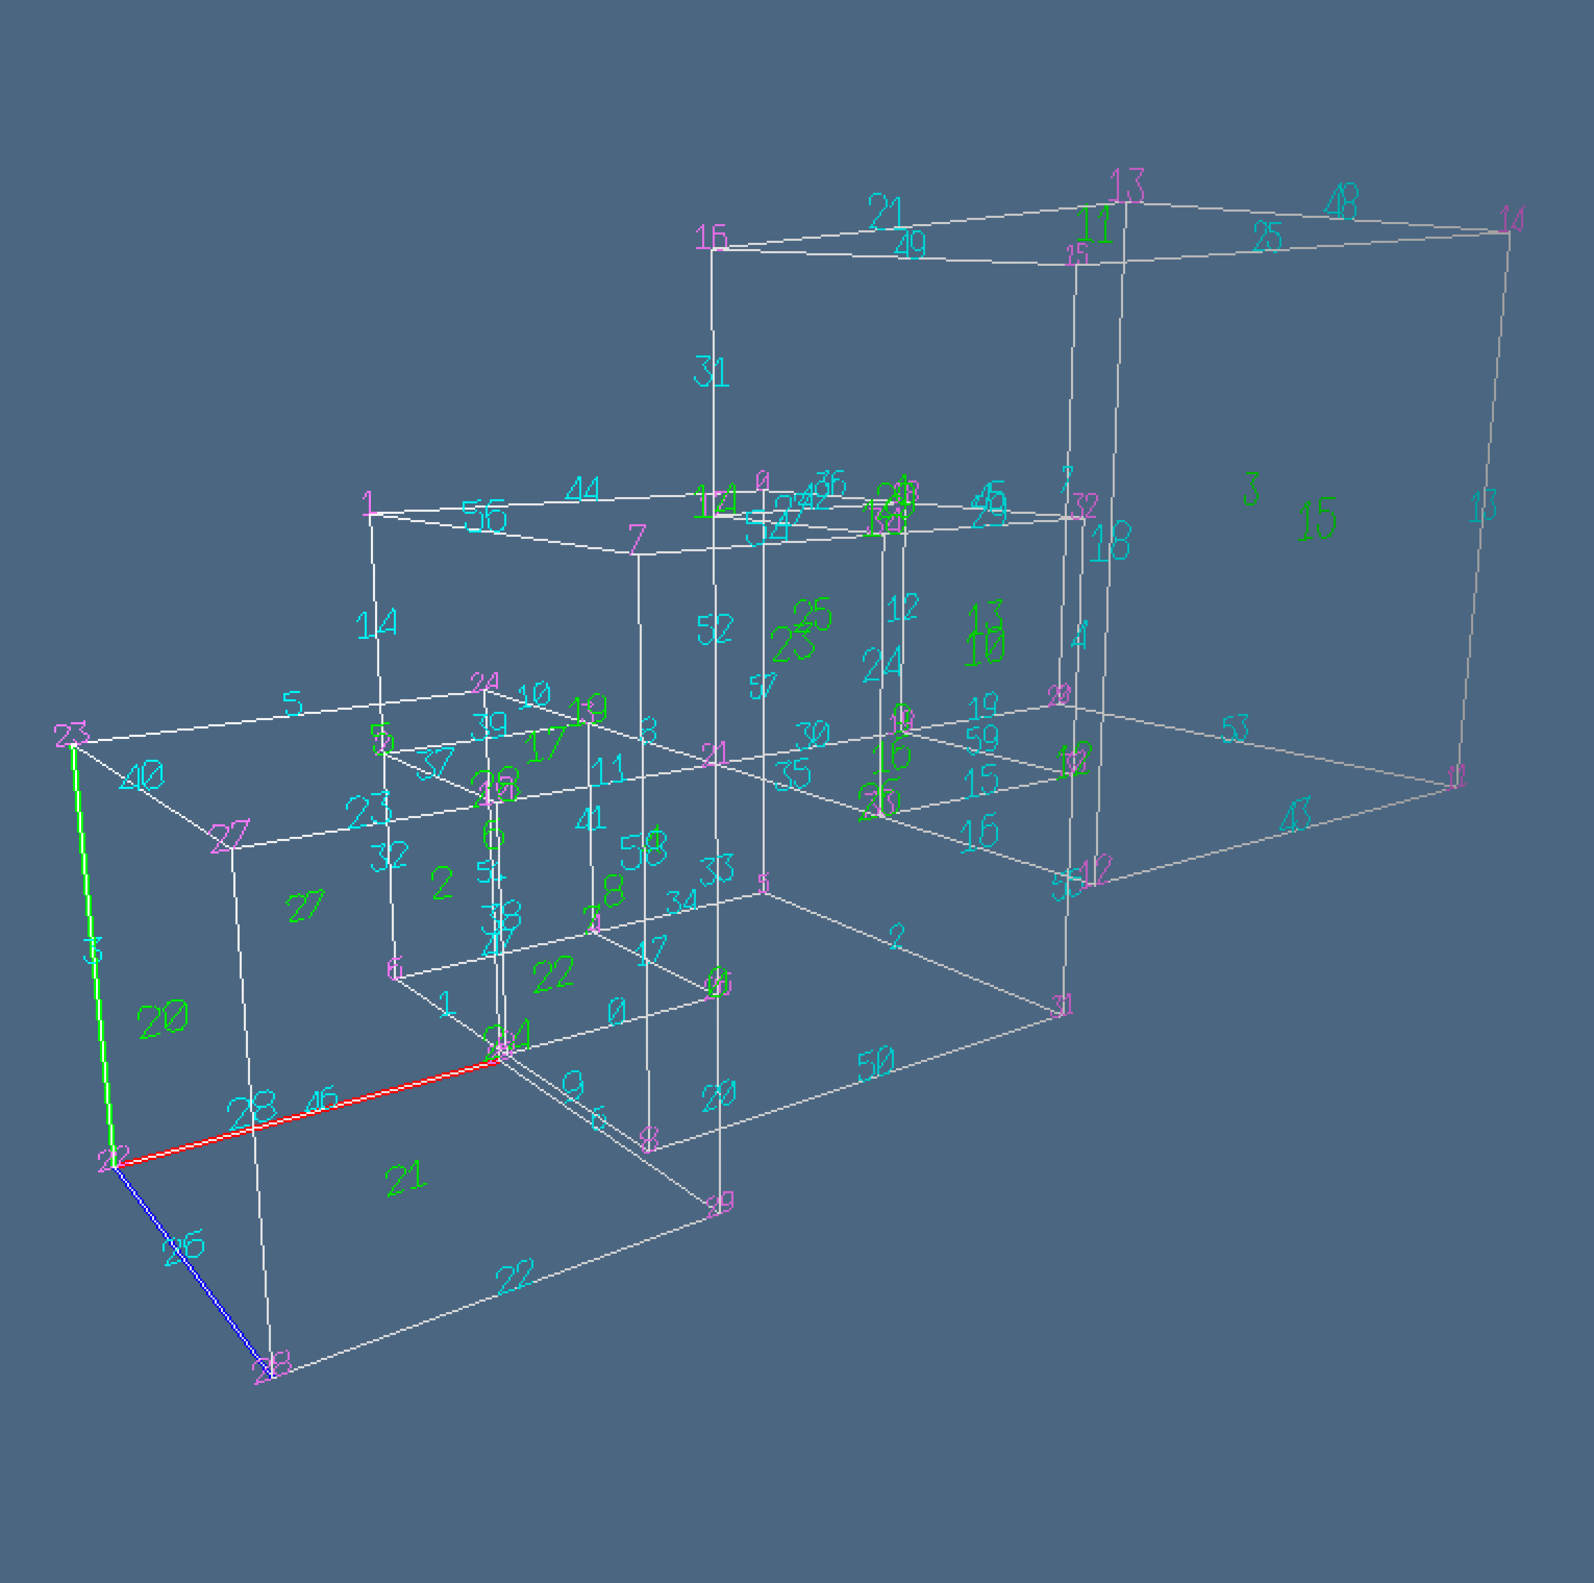
\includegraphics[height=0.332\textwidth,width=0.32\textwidth]{images/test11a1} 
   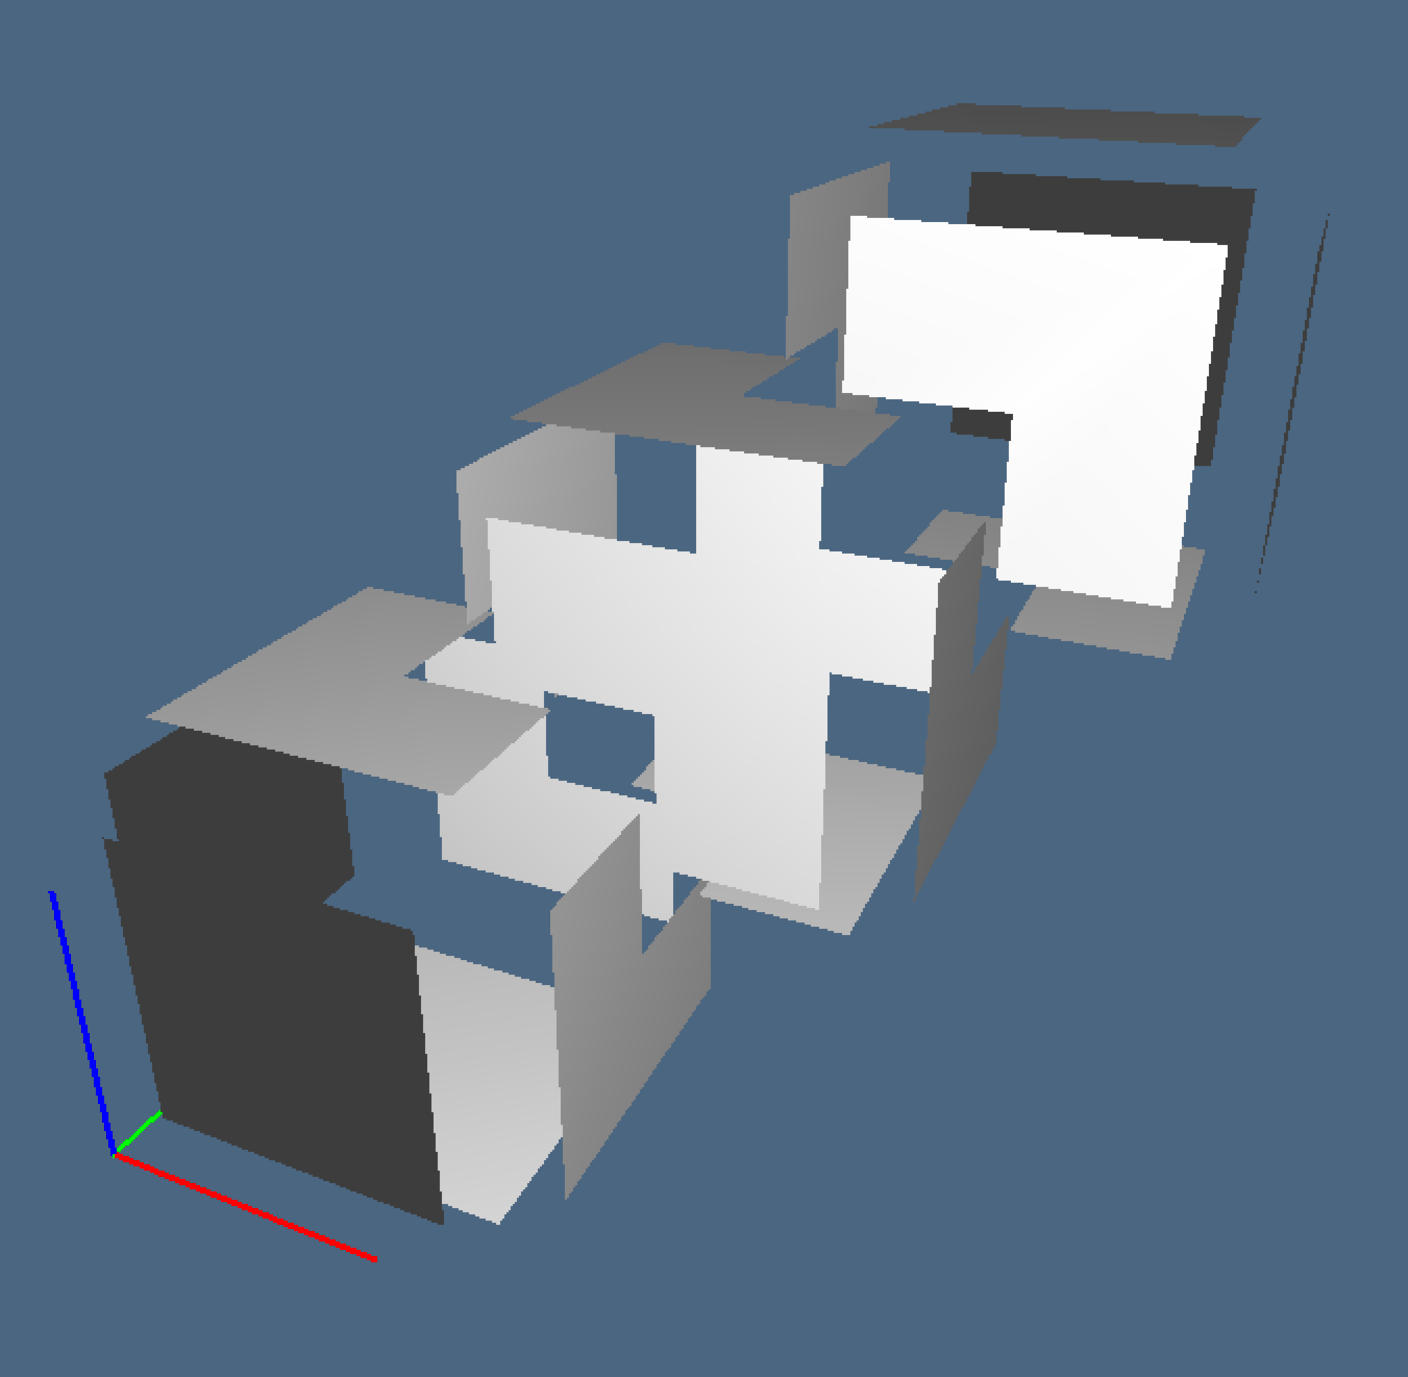
\includegraphics[height=0.332\textwidth,width=0.32\textwidth]{images/test11a2} 
   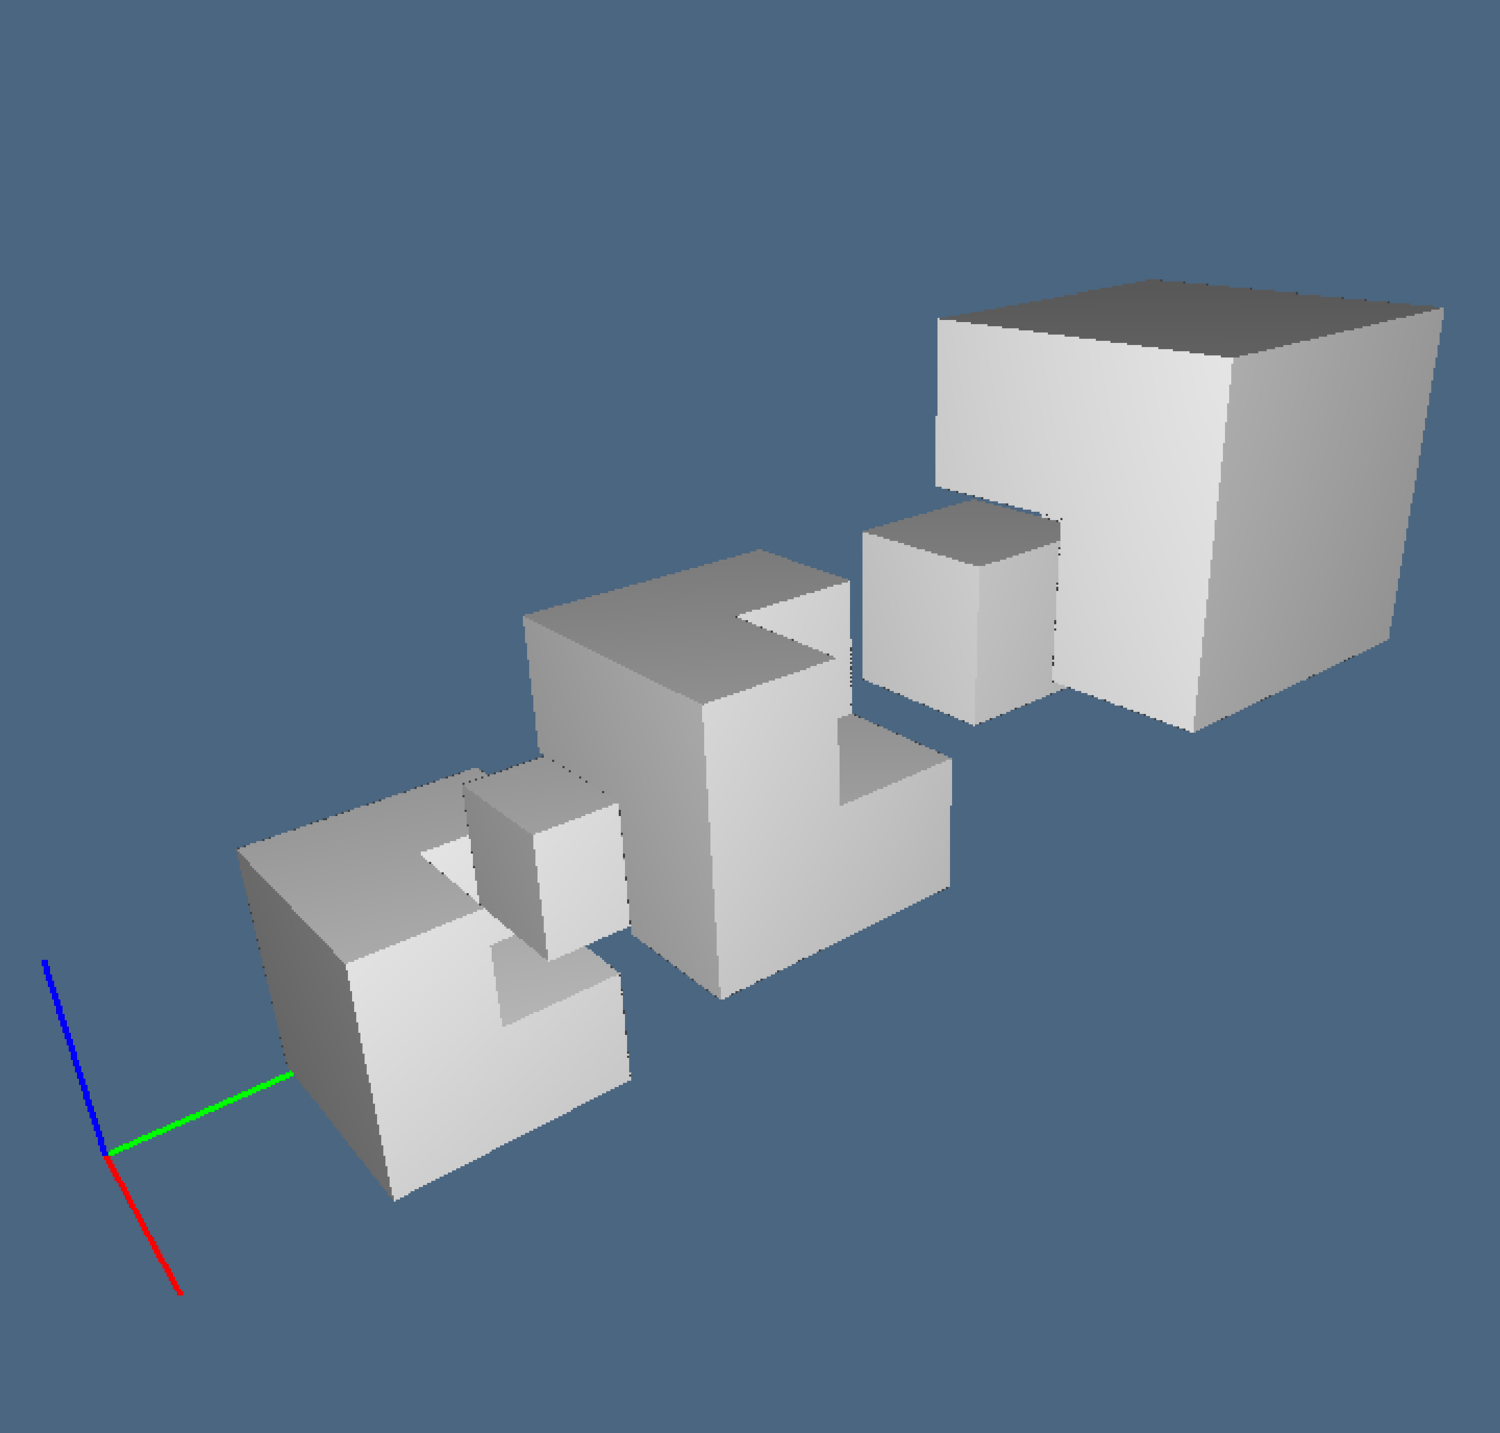
\includegraphics[height=0.332\textwidth,width=0.32\textwidth]{images/test11a3} 

   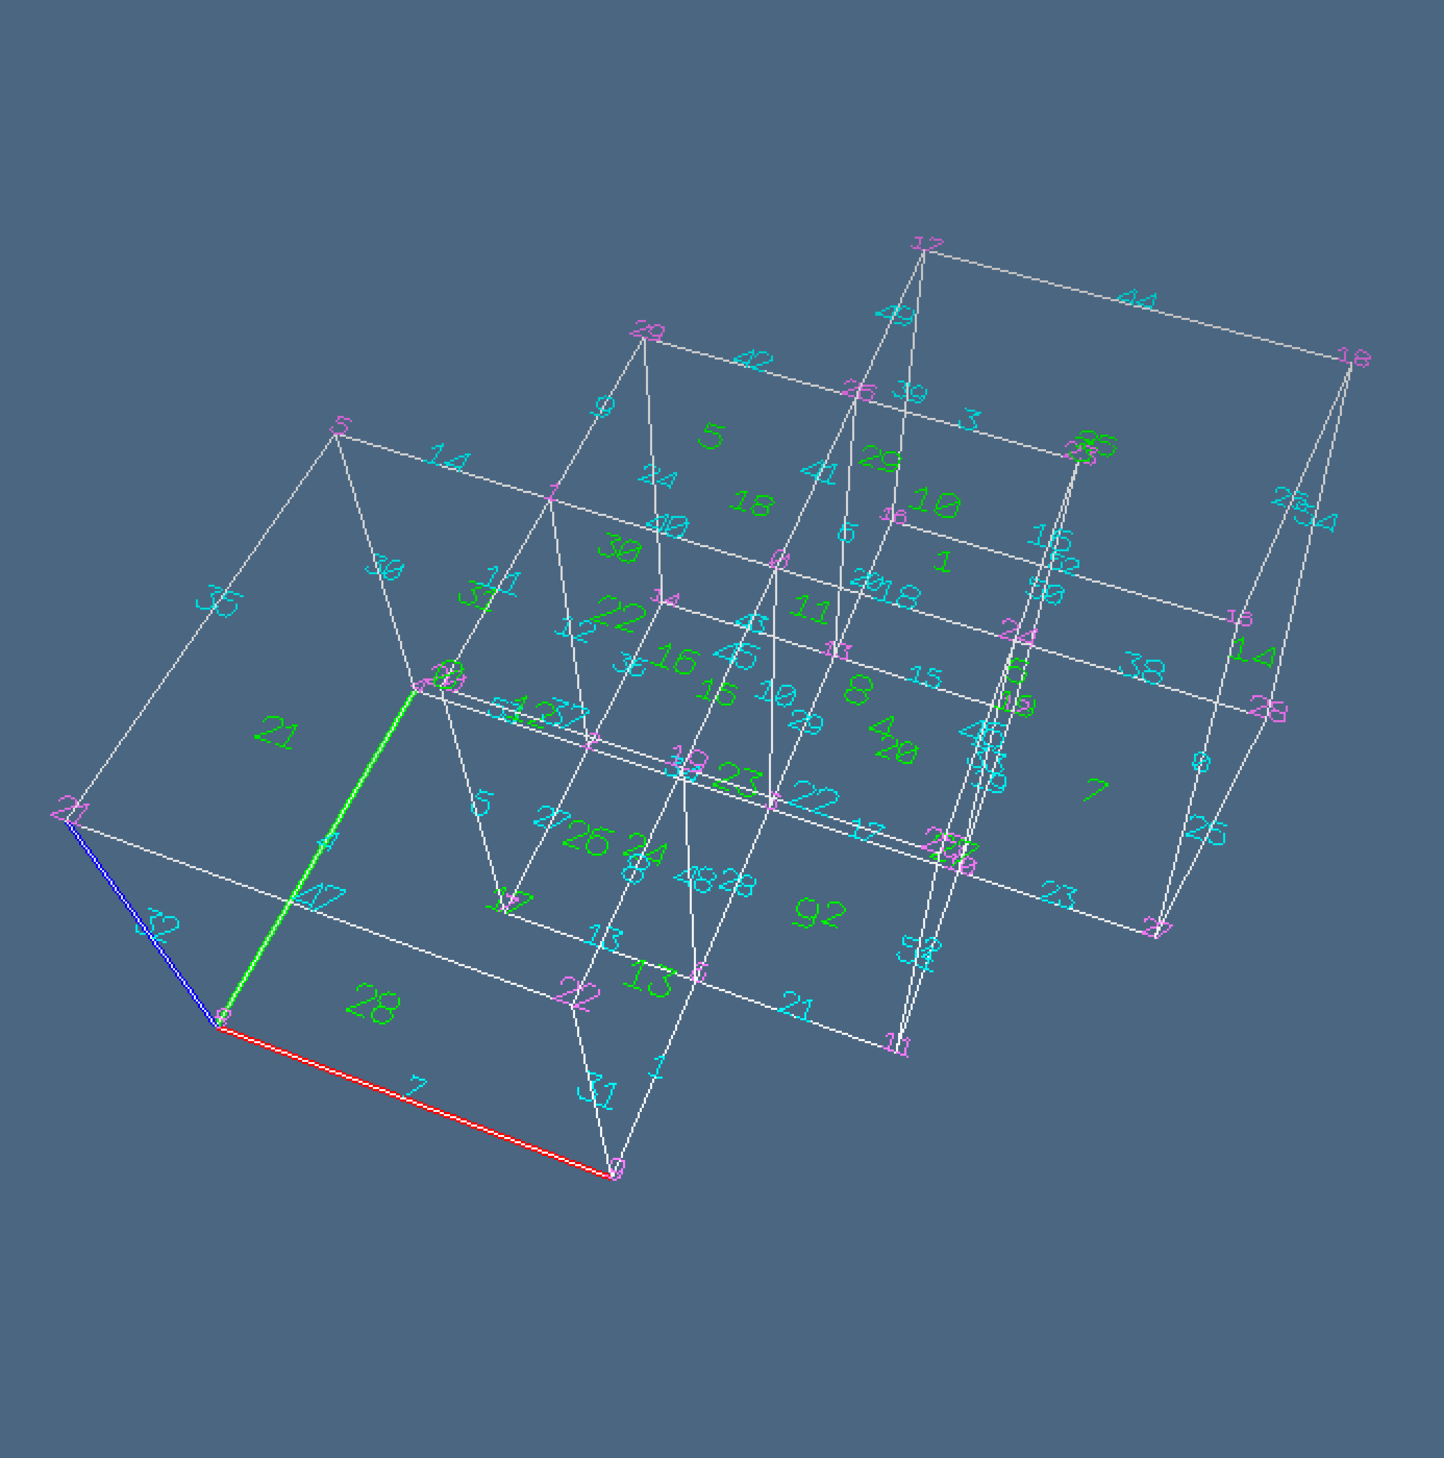
\includegraphics[height=0.332\textwidth,width=0.32\textwidth]{images/test11b1} 
   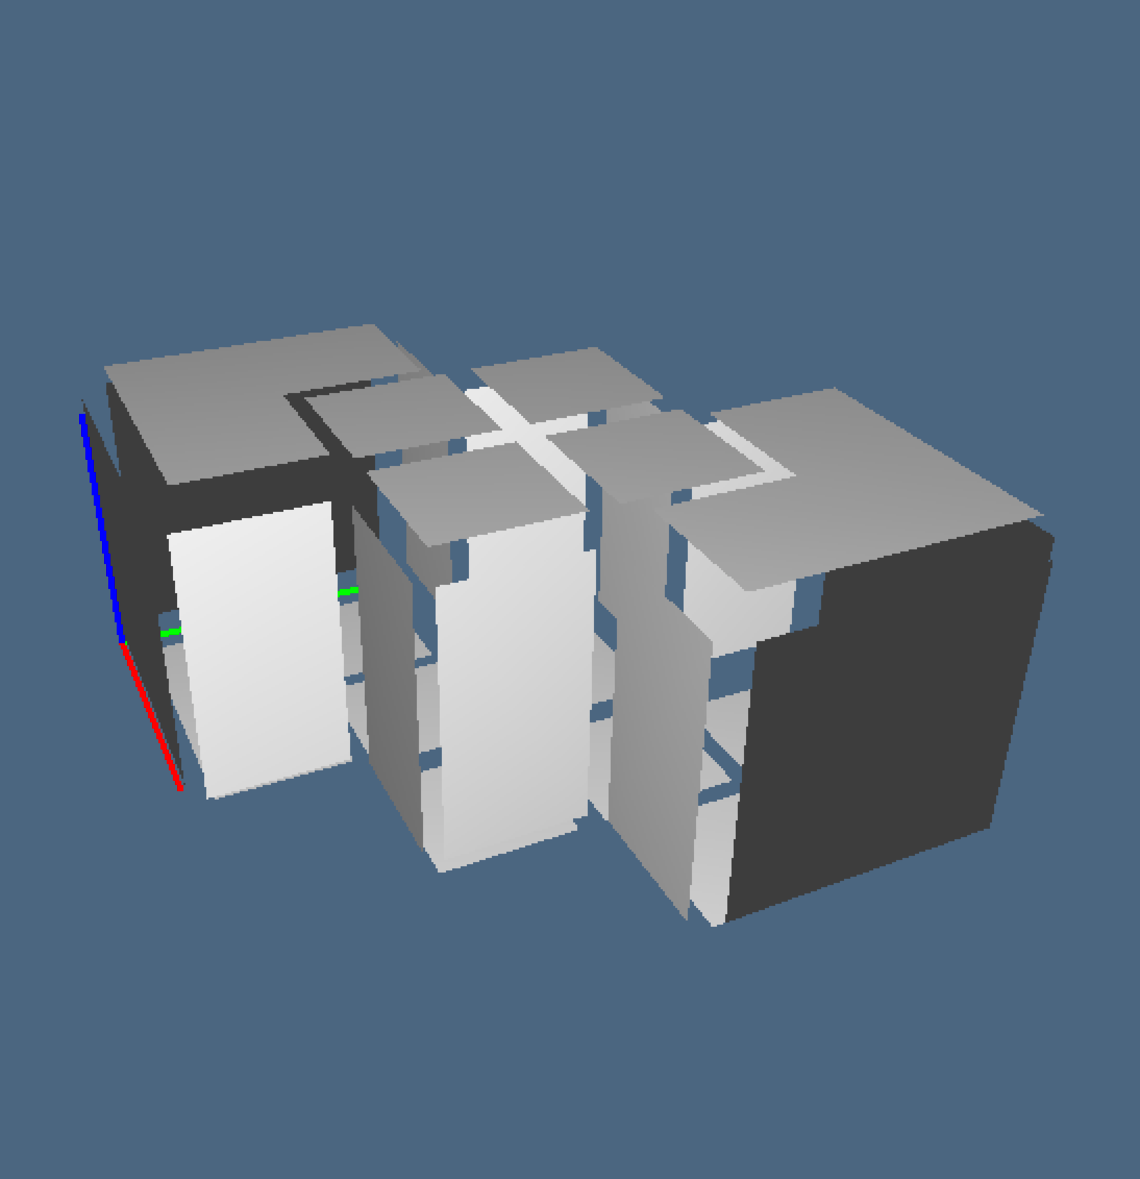
\includegraphics[height=0.332\textwidth,width=0.32\textwidth]{images/test11b2} 
   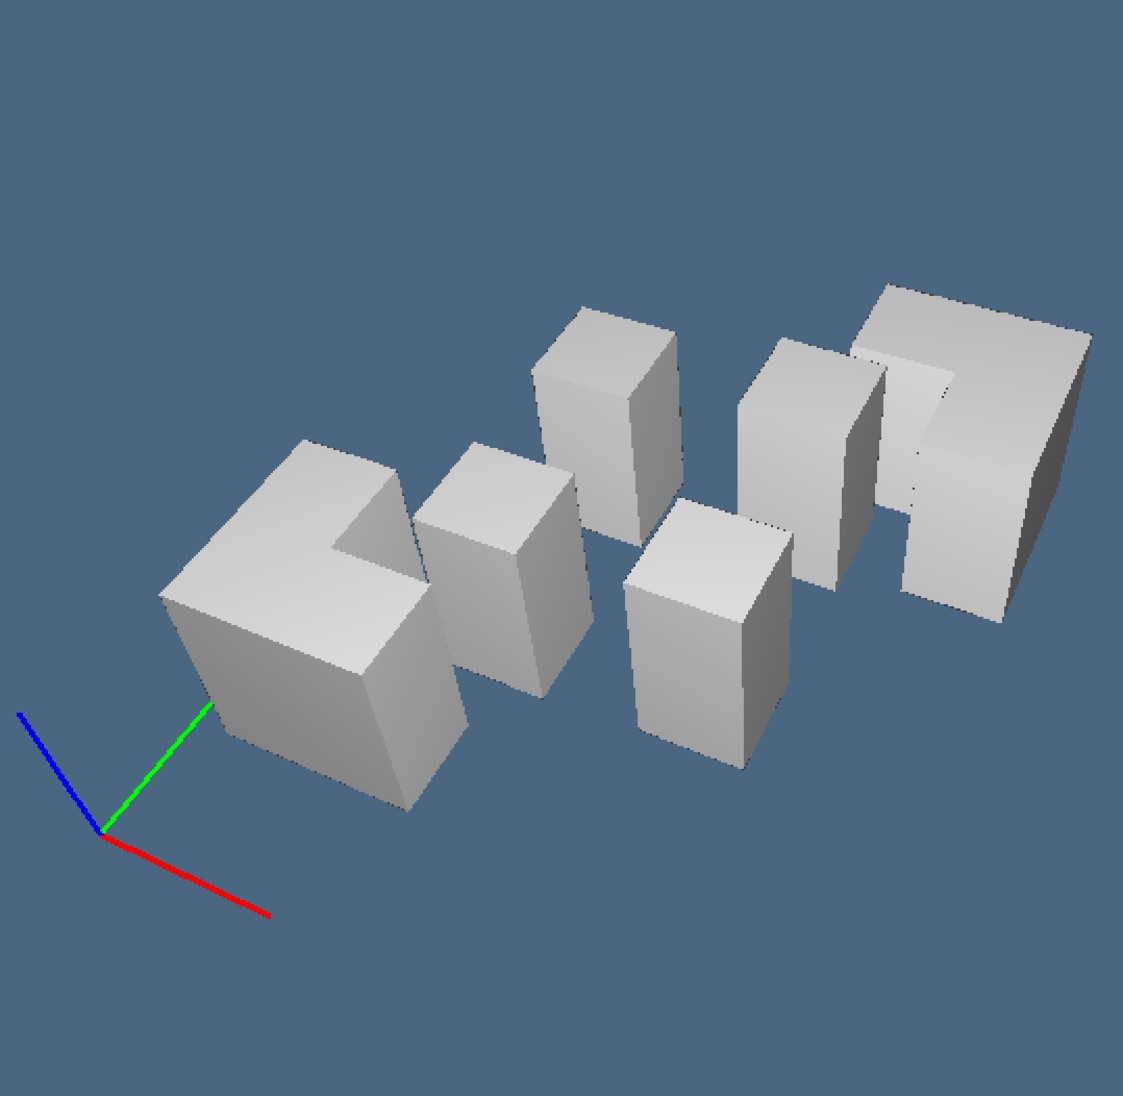
\includegraphics[height=0.332\textwidth,width=0.32\textwidth]{images/test11b3} 

   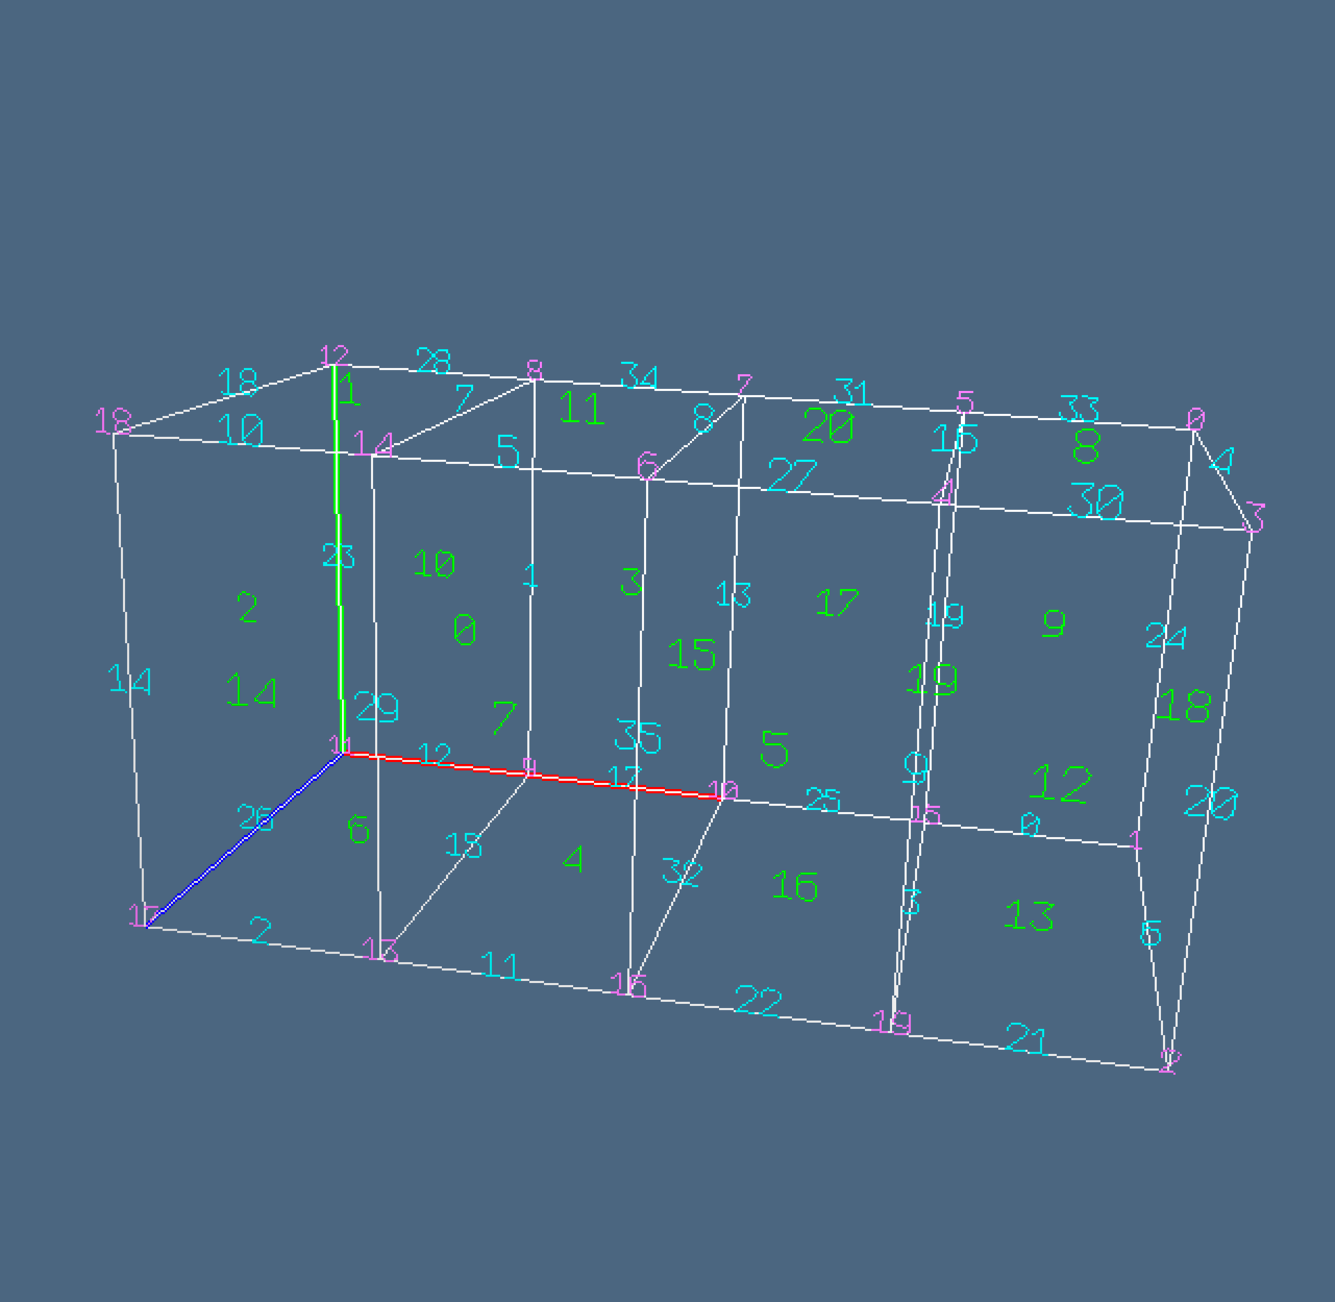
\includegraphics[height=0.332\textwidth,width=0.32\textwidth]{images/test11c1} 
   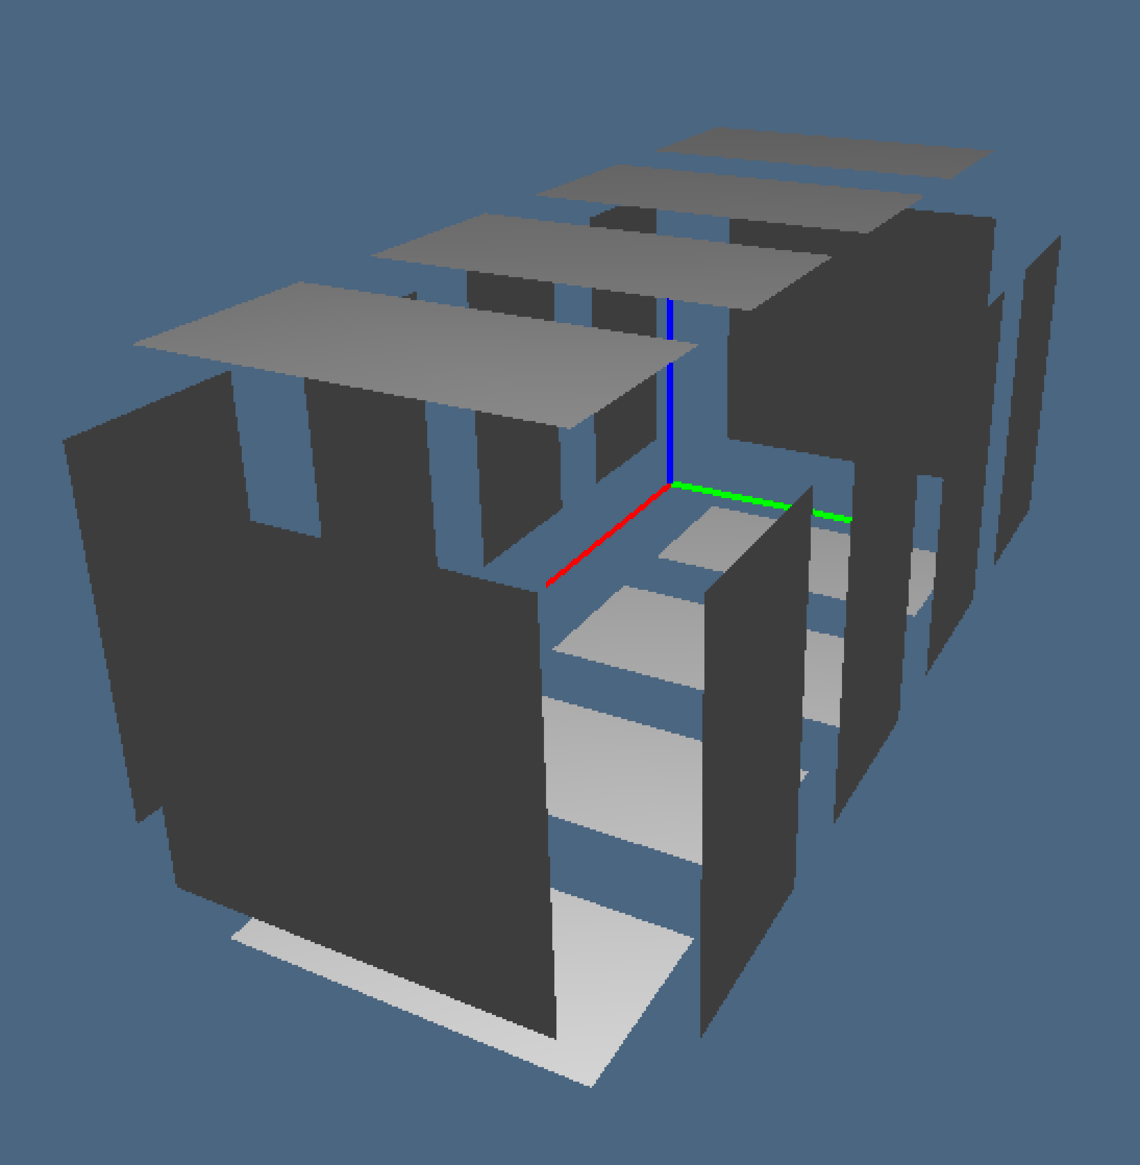
\includegraphics[height=0.332\textwidth,width=0.32\textwidth]{images/test11c2} 
   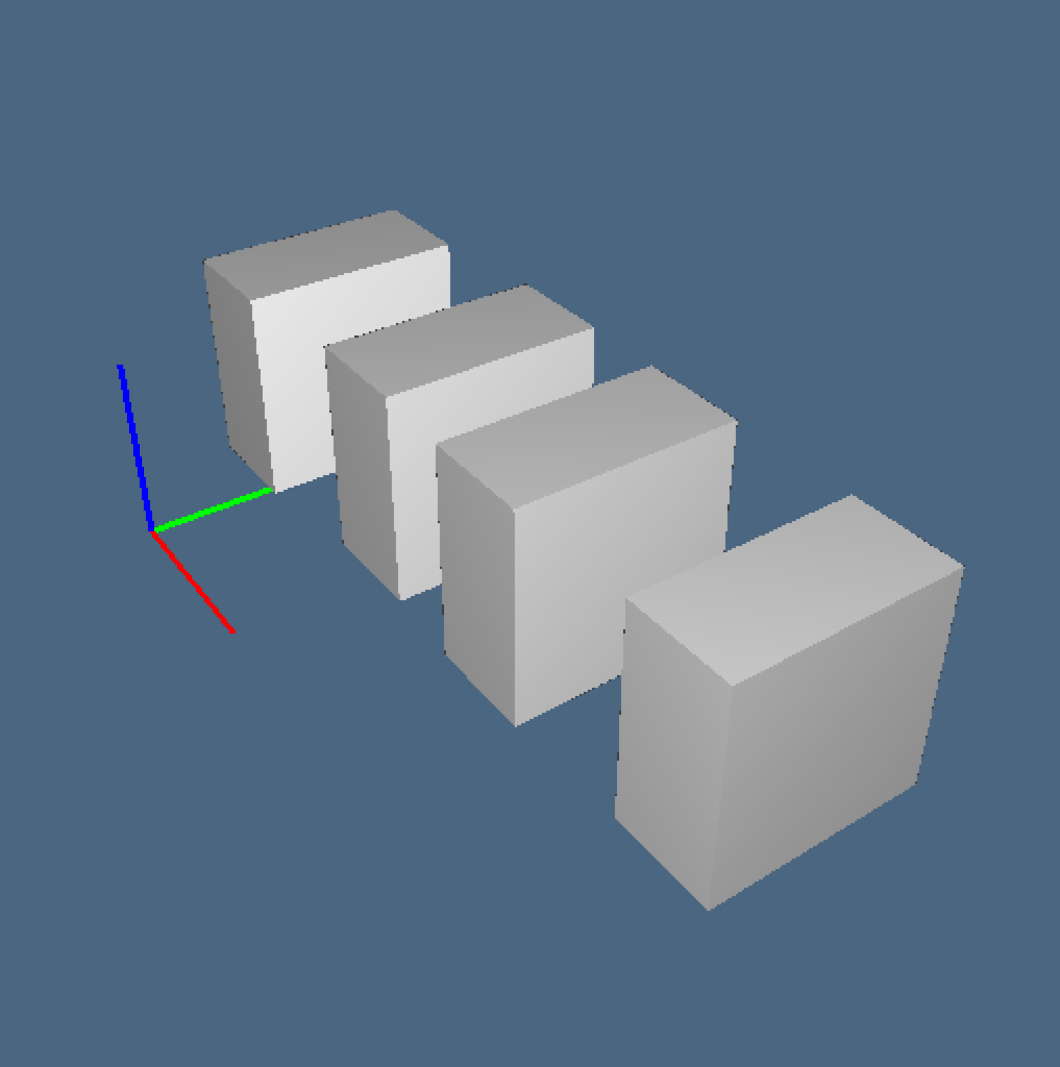
\includegraphics[height=0.332\textwidth,width=0.32\textwidth]{images/test11c3} 
   \caption{Examples of 3-cell extraction of two simple Boolean 2-complex, and their boundaries. Notice the numbers of (solid) 3-cells.}
   \label{fig:example}
\end{figure}


%-------------------------------------------------------------------------------
@O test/py/bool/test12.py @{
""" Testing of point-in-polygon classification algorithm """
from larlib import *

sys.path.insert(0, 'test/py/inters/')
from test10 import *

@< Point in polygon testing @>

result = []
for k in range(10000):
    queryPoint = [random.random(),random.random()]
    inOut = pointInPolygonClassification(queryPoint,[V,EV])
    #print k,queryPoint,inOut
    if inOut=="p_in": result += [MK(queryPoint)]
    elif inOut=="p_out": result += [COLOR(RED)(MK(queryPoint))]

VV = AA(LIST)(range(len(V)))
submodel = STRUCT(MKPOLS((V,EV)))
VIEW(STRUCT([
    POLYLINE([[queryPoint[0],0],[queryPoint[0],1]]),
    POLYLINE([[0,queryPoint[1]],[1,queryPoint[1]]]),
    larModelNumbering(1,1,1)(V,[VV,EV,FV[:-1]],submodel,0.4)
    ]+result))
@}
%-------------------------------------------------------------------------------

\begin{figure}[htbp] %  figure placement: here, top, bottom, or page
   \centering
   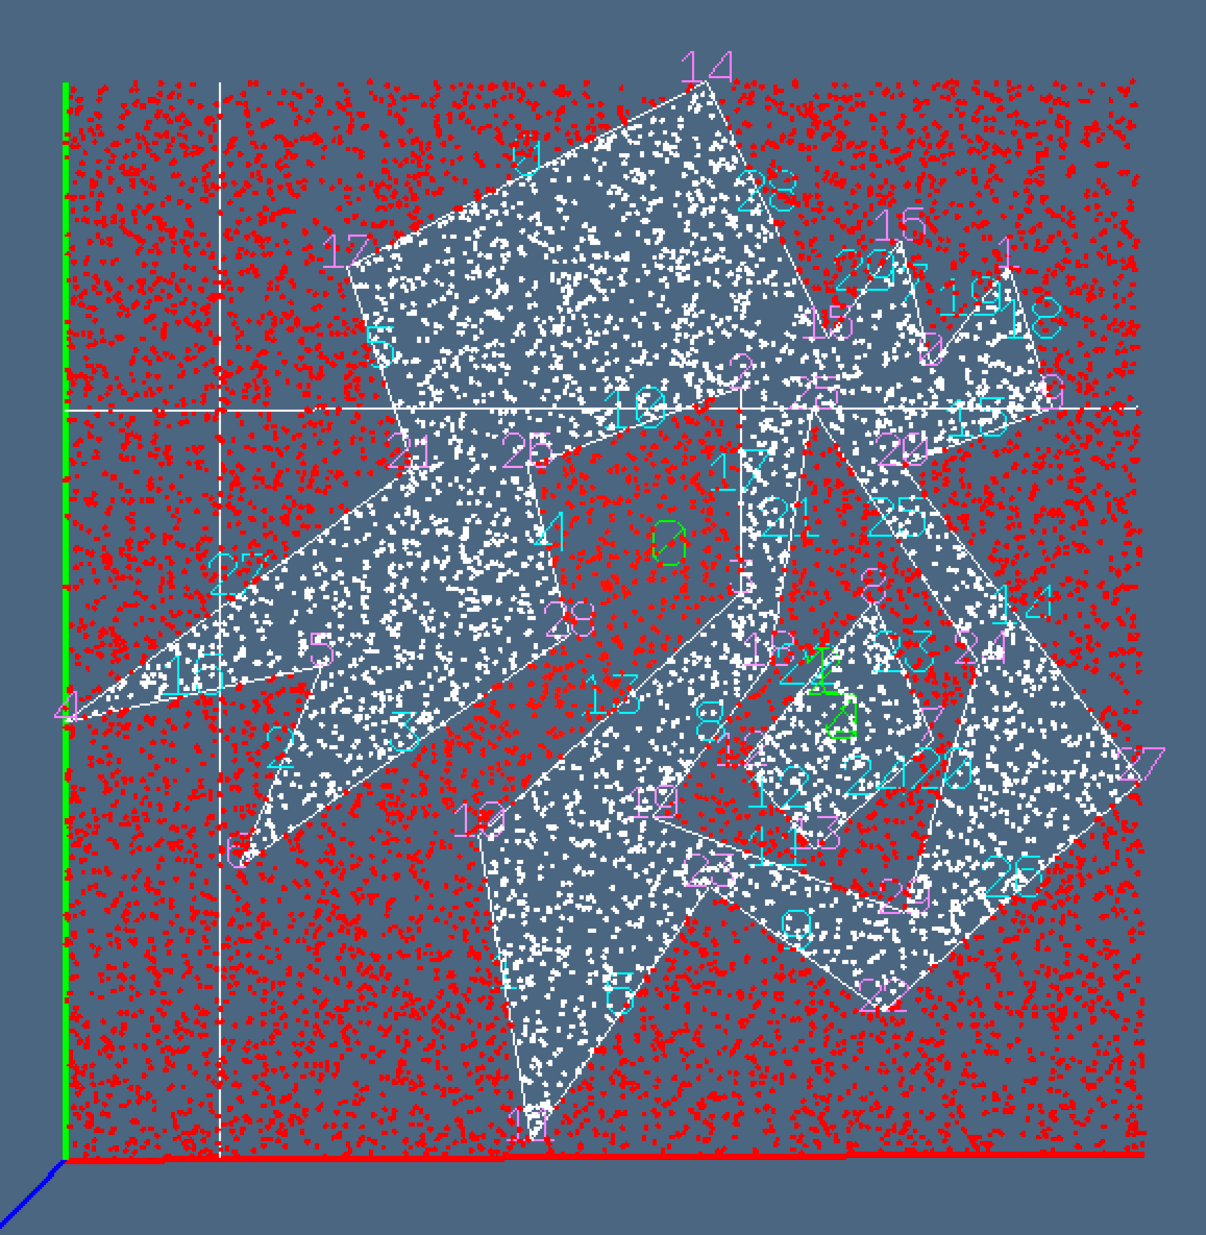
\includegraphics[width=0.5\linewidth]{images/pointInPolygon} 
   \caption{Testing the point-in-polygon algorithm.}
   \label{fig:pointInPolygon}
\end{figure}

\appendix
%===============================================================================
\section{Code utilities}
%===============================================================================

\subsection{Generation of random data}

Some utility fuctions used by the module are collected in this appendix. Their macro names can be seen in the below script.

%-------------------------------------------------------------------------------
@D Coding utilities
@{""" Coding utilities """
global count
@< Generation of a random 3D point @>
@< Generation of random 3D triangles @>
@< Generation of random 3D quadrilaterals @>
@< Generation of a single random triangle @>
@< Containment boxes @>
@< Transformation of a 3D box into an hexahedron @>
@< Computation of the 1D centroid of a list of 3D boxes @>
@< Generation of a list of HPCs from a LAR model with non-convex faces @>
@}
%-------------------------------------------------------------------------------


\paragraph{Generation of a list of HPCs from a LAR model with non-convex faces}

%-------------------------------------------------------------------------------
@D Generation of a list of HPCs from a LAR model with non-convex faces
@{""" Generation of a list of HPCs from a LAR model with non-convex faces """
def MKTRIANGLES(*model): 
    V,FV,EV = model
    FE = crossRelation(FV,EV)
    triangleSets = boundaryTriangulation(V,FV,EV,FE)
    return [ STRUCT([MKPOL([verts,[[1,2,3]],None]) for verts in triangledFace]) 
        for triangledFace in triangleSets ]

def MKSOLID(*model): 
    V,FV,EV = model
    FE = crossRelation(FV,EV)
    pivot = V[0]
    VF = invertRelation(FV) 
    faces = [face for face in FV if face not in VF[0]]
    triangleSets = boundaryTriangulation(V,faces,EV,FE)
    return XOR([ MKPOL([face+[pivot], [range(1,len(face)+2)],None])
        for face in CAT(triangleSets) ])
@}
%-------------------------------------------------------------------------------


\paragraph{Generation of random triangles}
The function \texttt{randomTriangles} returns the array \texttt{randomTriaArray} with a given number of triangles generated within the unit 3D interval. The \texttt{scaling} parameter is used to scale every such triangle, generated by three randow points, that could be possibly located to far from each other, even at the distance of the diagonal of the unit cube.

The arrays \texttt{xs}, \texttt{ys} and \texttt{zs}, that contain the $x,y,z$ coordinates of triangle points, are used to compute the minimal translation \texttt{v} needed to transport the entire set of data within the positive octant of the 3D space. 

%-------------------------------------------------------------------------------
@D Generation of random 3D triangles
@{""" Generation of random triangles """
def randomTriangles(numberOfTriangles=400,scaling=0.3):
    randomTriaArray = [rtriangle(scaling) for k in range(numberOfTriangles)]
    [xs,ys,zs] = TRANS(CAT(randomTriaArray))
    xmin, ymin, zmin = min(xs), min(ys), min(zs)
    v = array([-xmin,-ymin, -zmin])
    randomTriaArray = [[list(v1+v), list(v2+v), list(v3+v)] for v1,v2,v3 in randomTriaArray]
    return randomTriaArray
@}
%-------------------------------------------------------------------------------

\paragraph{Generation of random 3D quadrilaterals}

%-------------------------------------------------------------------------------
@D Generation of random 3D quadrilaterals
@{""" Generation of random 3D quadrilaterals """
def randomQuads(numberOfQuads=400,scaling=0.3):
    randomTriaArray = [rtriangle(scaling) for k in range(numberOfQuads)]
    [xs,ys,zs] = TRANS(CAT(randomTriaArray))
    xmin, ymin, zmin = min(xs), min(ys), min(zs)
    v = array([-xmin,-ymin, -zmin])
    randomQuadArray = [AA(list)([ v1+v, v2+v, v3+v, v+v2-v1+v3 ]) for v1,v2,v3 in randomTriaArray]
    return randomQuadArray
@}
%-------------------------------------------------------------------------------


\paragraph{Generation of a random 3D point}
A single random point, codified in floating point format, and with a fixed (quite small) number of digits, is returned by the \texttt{rpoint()} function, with no input parameters.
%-------------------------------------------------------------------------------
@D Generation of a random 3D point
@{""" Generation of a random 3D point """
def rpoint():
    return eval( vcode([ random.random(), random.random(), random.random() ]) )
@}
%-------------------------------------------------------------------------------
    
\paragraph{Generation of a single random triangle}
A single random triangle, scaled about its centroid by the \texttt{scaling} parameter, is returned by the \texttt{rtriangle()} function, as a tuple ot two random points in the unit square.
%-------------------------------------------------------------------------------
@D Generation of a single random triangle
@{""" Generation of a single random triangle """
def rtriangle(scaling):
    v1,v2,v3 = array(rpoint()), array(rpoint()), array(rpoint())
    c = (v1+v2+v3)/3
    pos = rpoint()
    v1 = (v1-c)*scaling + pos
    v2 = (v2-c)*scaling + pos
    v3 = (v3-c)*scaling + pos
    return tuple(eval(vcode(v1))), tuple(eval(vcode(v2))), tuple(eval(vcode(v3)))
@}
%-------------------------------------------------------------------------------
    

\paragraph{Containment boxes}

Given as input a list \texttt{randomTriaArray} of pairs of 2D points, the function \texttt{containmentBoxes} returns, in the same order, the list of \emph{containment boxes} of the input lines. A \emph{containment box} of a geometric object of dimension $d$ is defined as the minimal $d$-cuboid, equioriented with the reference frame, that contains the object. For a 2D line it is given by the tuple $(x1,y1,x2,y2)$, where $(x1,y1)$ is the point of minimal coordinates, and $(x2,y2)$ is the point of maximal  coordinates.

%-------------------------------------------------------------------------------
@D Containment boxes
@{""" Containment boxes """
def containmentBoxes(randomPointArray,qualifier=0):
    if len(randomPointArray[0])==2:
        boxes = [eval(vcode([min(x1,x2), min(y1,y2), min(z1,z2), 
                             max(x1,x2), max(y1,y2), max(z1,z2)]))+[qualifier]
                for ((x1,y1,z1),(x2,y2,z2)) in randomPointArray]
    elif len(randomPointArray[0])==3:
        boxes = [eval(vcode([min(x1,x2,x3), min(y1,y2,y3), min(z1,z2,z3), 
                             max(x1,x2,x3), max(y1,y2,y3), max(z1,z2,z3)]))+[qualifier]
                for ((x1,y1,z1),(x2,y2,z2),(x3,y3,z3)) in randomPointArray]
    elif len(randomPointArray[0])==4:
        boxes = [eval(vcode([min(x1,x2,x3,x4), min(y1,y2,y3,y4), min(z1,z2,z3,z4), 
                             max(x1,x2,x3,x4), max(y1,y2,y3,y4), max(z1,z2,z3,z4)]))+[qualifier]
                for ((x1,y1,z1),(x2,y2,z2),(x3,y3,z3),(x4,y4,z4)) in randomPointArray]
    return boxes
@}
%-------------------------------------------------------------------------------

    
\paragraph{Transformation of a 3D box into an hexahedron}
The transformation of a 2D box into a closed rectangular polyline, given as an ordered sequwncw of 2D points, is produced by the function \texttt{box2exa}
%-------------------------------------------------------------------------------
@D Transformation of a 3D box into an hexahedron
@{""" Transformation of a 3D box into an hexahedron """    
def box2exa(box):
    x1,y1,z1,x2,y2,z2,type = box
    verts = [[x1,y1,z1], [x1,y1,z2], [x1,y2,z1], [x1,y2,z2], [x2,y1,z1], [x2,y1,z2], [x2,y2,z1], [x2,y2,z2]]
    cell = [range(1,len(verts)+1)]
    return [verts,cell,None],type

def lar2boxes(model,qualifier=0):
    V,CV = model
    boxes = []
    for k,cell in enumerate(CV):
        verts = [V[v] for v in cell]
        x1,y1,z1 = [min(coord) for coord in TRANS(verts)]
        x2,y2,z2 = [max(coord) for coord in TRANS(verts)]
        boxes += [eval(vcode([min(x1,x2),min(y1,y2),min(z1,z2),max(x1,x2),max(y1,y2),max(z1,z2)]))+[(qualifier,k)]]
    return boxes
@}
%-------------------------------------------------------------------------------
    
\paragraph{Computation of the 1D centroid of a list of 3D boxes}
The 1D \texttt{centroid} of a list of 3D boxes is computed by the function given below.
The direction of computation (either $x,y$ or $z$) is chosen depending on the value of the \texttt{coord} parameter. 
%-------------------------------------------------------------------------------
@D Computation of the 1D centroid of a list of 3D boxes
@{""" Computation of the 1D centroid of a list of 3D boxes """    
def centroid(boxes,coord):
    delta,n = 0,len(boxes)
    ncoords = len(boxes[0])/2
    a = coord%ncoords
    b = a+ncoords
    for box in boxes:
        delta += (box[a] + box[b])/2
    return delta/n
@}
%-------------------------------------------------------------------------------

\subsection{Point in polygon classification}

%-------------------------------------------------------------------------------
@D Point in polygon testing
@{
@< Half-line crossing test @>
@< Tile codes computation @>
@< Point-in-polygon classification algorithm @>
@}
%-------------------------------------------------------------------------------

\paragraph{Tile codes computation}
%-------------------------------------------------------------------------------
@D Tile codes computation
@{""" Tile codes computation """
def setTile(box):
    tiles = [[9,1,5],[8,0,4],[10,2,6]]
    b1,b2,b3,b4 = box
    def tileCode(point):
        x,y = point
        code = 0
        if y>b1: code=code|1
        if y<b2: code=code|2
        if x>b3: code=code|4
        if x<b4: code=code|8
        return code 
    return tileCode
@}
%-------------------------------------------------------------------------------

\paragraph{Point in polygon testing}
%-------------------------------------------------------------------------------
@D Point-in-polygon classification algorithm
@{""" Point in polygon classification """
def pointInPolygonClassification(p,pol):
    x,y = p
    V,EV = pol
    xmin,xmax,ymin,ymax = x,x,y,y
    tilecode = setTile([ymax,ymin,xmax,xmin])
    count,status = 0,0
    for k,edge in enumerate(EV):
        p1,p2 = V[edge[0]],V[edge[1]]
        (x1,y1),(x2,y2) = p1,p2
        c1,c2 = tilecode(p1),tilecode(p2)
        k,c_edge, c_un, c_int = k,c1^c2, c1|c2, c1&c2
        #print "k,c_edge, c_un, c_int =",k,c_edge, c_un, c_int
        
        if c_edge == 0 and c_un == 0: return "p_on"
        elif c_edge == 12 and c_un == c_edge: return "p_on"
        elif c_edge == 3:
            if c_int == 0: return "p_on"
            elif c_int == 4: count += 1
        elif c_edge == 15:
            x_int = ((y-y2)*(x1-x2)/(y1-y2))+x2 
            if x_int > x: count += 1
            elif x_int == x: return "p_on"
        elif c_edge == 13 and ((c1==4) or (c2==4)):
                count,status = crossingTest(1,2,count,status)
        elif c_edge == 14 and (c1==4) or (c2==4):
                count,status = crossingTest(2,1,count,status)
        elif c_edge == 7: count += 1
        elif c_edge == 11: count = count
        elif c_edge == 1:
            if c_int == 0: return "p_on"
            elif c_int == 4: count,status = crossingTest(1,2,count,status)
        elif c_edge == 2:
            if c_int == 0: return "p_on"
            elif c_int == 4: count,status = crossingTest(2,1,count,status)
        elif c_edge == 4 and c_un == c_edge: return "p_on"
        elif c_edge == 8 and c_un == c_edge: return "p_on"
        elif c_edge == 5:
            if (c1==0) or (c2==0): return "p_on"
            else: count,status = crossingTest(1,2,count,status)
        elif c_edge == 6:
            if (c1==0) or (c2==0): return "p_on"
            else: count,status = crossingTest(2,1,count,status)
        elif c_edge == 9 and ((c1==0) or (c2==0)): return "p_on"
        elif c_edge == 10 and ((c1==0) or (c2==0)): return "p_on"
        #print "count,p1,p2 =",count,p1,p2        
    if (round(count)%2)==1: return "p_in"
    else: return "p_out"
@}
%-------------------------------------------------------------------------------

\paragraph{Half-line crossing test}
%-------------------------------------------------------------------------------
@D Half-line crossing test 
@{""" Half-line crossing test """
def crossingTest(new,old,count,status):
    if status == 0:
        status = new
        count += 0.5
    else:
        if status == old: count += 0.5
        else: count -= 0.5
        status = 0
    return count,status
@}
%-------------------------------------------------------------------------------

\bibliographystyle{amsalpha}
\bibliography{bool}

\end{document}
